%%%%%%%%%%%%%%%%%%%%%%%%%%%%%%%%%%%%%%%%%%%%%%%%%%%%%%%%%%%

%%%%%%%%%%%%%%%%%%%%%%%%%%%%%%%%%%%%%%%%%%%%%%%%%%%%%%%%%%%

%% document class
\documentclass[a4paper,11pt,oneside]{book}

%% packages
%% packages

\usepackage{blindtext} % needed for creating dummy text passages
%\usepackage{ngerman} % needed for German default language
\usepackage{amsmath} % needed for command eqref
\usepackage{amssymb} % needed for math fonts
\usepackage[
	colorlinks=true
	,breaklinks
	%,ngerman
	]{hyperref} % needed for creating hyperlinks in the document, the option colorlinks=true gets rid of the awful boxes, breaklinks breaks lonkg links (list of figures), and ngerman sets everything for german as default hyperlinks language
\usepackage[hyphenbreaks]{breakurl} % ben�tigt f�r das Brechen von URLs in Literaturreferenzen, hyphenbreaks auch bei links, die �ber eine Seite gehen (mit hyphenation).
\usepackage{xcolor}
\definecolor{c1}{rgb}{0,0,1} % blue
\definecolor{c2}{rgb}{0,0.3,0.9} % light blue
\definecolor{c3}{rgb}{0.3,0,0.9} % red blue
\hypersetup{
    linkcolor={c1}, % internal links
    citecolor={c2}, % citations
    urlcolor={c3} % external links/urls
}
%\usepackage{cite} % needed for cite
\usepackage[round,authoryear]{natbib} % needed for cite and abbrvnat bibliography style
\usepackage[nottoc]{tocbibind} % needed for displaying bibliography and other in the table of contents
\usepackage{graphicx} % needed for \includegraphics 
\usepackage{longtable} % needed for long tables over pages
\usepackage{bigstrut} % needed for the command \bigstrut
\usepackage{enumerate} % needed for some options in enumerate
\usepackage{array}
\usepackage{textgreek}
\usepackage{todonotes} % needed for todos
\usepackage{makeidx} % needed for creating an index
\makeindex
\usepackage{placeins}
\usepackage [english]{babel}
\usepackage [autostyle, english = american]{csquotes}
\MakeOuterQuote{"}
\usepackage{multirow}
\usepackage{dcolumn}
\usepackage{array}
\usepackage{makecell}

%% page settings
%% page settings

\usepackage[top=2cm, bottom=1.8cm,left=2.5cm,right=2.5cm]{geometry} % needed for page border settings
\parindent=0cm % for space of first line of new text block
\sloppy % for writing with hyphenless justification (tries to)
\hyphenation{} % use hyphenation of tolerance parameters, http://www.jr-x.de/publikationen/latex/tipps/zeilenumbruch.html
\hyphenpenalty=10000
\exhyphenpenalty=10000
\usepackage{fancyhdr} % needed for head and foot options

%% own commands
%\newcommand{\tbi}[1]{\textbf{\textit{#1}}}
%% my macros

%% Text fomats
\newcommand{\tbi}[1]{\textbf{\textit{#1}}}

%% Math fonts
\newcommand{\bbA}{\mathbb{A}}
\newcommand{\bbB}{\mathbb{B}}
\newcommand{\bbC}{\mathbb{C}}
\newcommand{\bbD}{\mathbb{D}}
\newcommand{\bbE}{\mathbb{E}}
\newcommand{\bbF}{\mathbb{F}}
\newcommand{\bbG}{\mathbb{G}}
\newcommand{\bbH}{\mathbb{H}}
\newcommand{\bbI}{\mathbb{I}}
\newcommand{\bbJ}{\mathbb{J}}
\newcommand{\bbK}{\mathbb{K}}
\newcommand{\bbL}{\mathbb{L}}
\newcommand{\bbM}{\mathbb{M}}
\newcommand{\bbN}{\mathbb{N}}
\newcommand{\bbO}{\mathbb{O}}
\newcommand{\bbP}{\mathbb{P}}
\newcommand{\bbQ}{\mathbb{Q}}
\newcommand{\bbR}{\mathbb{R}}
\newcommand{\bbS}{\mathbb{S}}
\newcommand{\bbT}{\mathbb{T}}
\newcommand{\bbU}{\mathbb{U}}
\newcommand{\bbV}{\mathbb{V}}
\newcommand{\bbW}{\mathbb{W}}
\newcommand{\bbX}{\mathbb{X}}
\newcommand{\bbY}{\mathbb{Y}}
\newcommand{\bbZ}{\mathbb{Z}}
\newcommand{\imp}[1]{\underline{\textit{#1}}}

%%%%%%%%%%%%%%%%%%%%%%%%%%%%%%%%%%%%%%%%%%%%%%%%%%%%%%%%%%%

\begin{document}
	
	%%%%%%%%%%%%%%%%%%%%%%%%%%%%%%%%%%%%%%%%%%%%%%%%%%%%%%%%%%%
	%%%%%%%%%%%%%%%%%%%%%%%%%%%%%%%%%%%%%%%%%%%%%%%%%%%%%%%%%%%
	%%%%%%%%%%%%%%%%%%%%%%%%%%%%%%%%%%%%%%%%%%%%%%%%%%%%%%%%%%%
	
	%\pagestyle{empty}
	%\title{Basic elements for writing a book/thesis using \LaTeX}
	%\autr{Mauricio Lobos}
	%\date{}
	%\maketitle
	%%%%%%%%%%%%%%%%%%%%%%%%%%%%%%%%%%%%%%%%%
% University Assignment Title Page 
% LaTeX Template
% Version 1.0 (27/12/12)
%
% This template has been downloaded from:
% http://www.LaTeXTemplates.com
%
% Original author:
% WikiBooks (http://en.wikibooks.org/wiki/LaTeX/Title_Creation)
%
% License:
% CC BY-NC-SA 3.0 (http://creativecommons.org/licenses/by-nc-sa/3.0/)
% 
% Instructions for using this template:
% This title page is capable of being compiled as is. This is not useful for 
% including it in another document. To do this, you have two options: 
%
% 1) Copy/paste everything between \begin{document} and \end{document} 
% starting at \begin{} and paste this into another LaTeX file where you 
% want your title page.
% OR
% 2) Remove everything outside the \begin{titlepage} and \end{titlepage} and 
% move this file to the same directory as the LaTeX file you wish to add it to. 
% Then add %%%%%%%%%%%%%%%%%%%%%%%%%%%%%%%%%%%%%%%%%
% University Assignment Title Page 
% LaTeX Template
% Version 1.0 (27/12/12)
%
% This template has been downloaded from:
% http://www.LaTeXTemplates.com
%
% Original author:
% WikiBooks (http://en.wikibooks.org/wiki/LaTeX/Title_Creation)
%
% License:
% CC BY-NC-SA 3.0 (http://creativecommons.org/licenses/by-nc-sa/3.0/)
% 
% Instructions for using this template:
% This title page is capable of being compiled as is. This is not useful for 
% including it in another document. To do this, you have two options: 
%
% 1) Copy/paste everything between \begin{document} and \end{document} 
% starting at \begin{} and paste this into another LaTeX file where you 
% want your title page.
% OR
% 2) Remove everything outside the \begin{titlepage} and \end{titlepage} and 
% move this file to the same directory as the LaTeX file you wish to add it to. 
% Then add %%%%%%%%%%%%%%%%%%%%%%%%%%%%%%%%%%%%%%%%%
% University Assignment Title Page 
% LaTeX Template
% Version 1.0 (27/12/12)
%
% This template has been downloaded from:
% http://www.LaTeXTemplates.com
%
% Original author:
% WikiBooks (http://en.wikibooks.org/wiki/LaTeX/Title_Creation)
%
% License:
% CC BY-NC-SA 3.0 (http://creativecommons.org/licenses/by-nc-sa/3.0/)
% 
% Instructions for using this template:
% This title page is capable of being compiled as is. This is not useful for 
% including it in another document. To do this, you have two options: 
%
% 1) Copy/paste everything between \begin{document} and \end{document} 
% starting at \begin{} and paste this into another LaTeX file where you 
% want your title page.
% OR
% 2) Remove everything outside the \begin{titlepage} and \end{titlepage} and 
% move this file to the same directory as the LaTeX file you wish to add it to. 
% Then add \input{./title_page_1.tex} to your LaTeX file where you want your
% title page.
%
%%%%%%%%%%%%%%%%%%%%%%%%%%%%%%%%%%%%%%%%%

%----------------------------------------------------------------------------------------
%	PACKAGES AND OTHER DOCUMENT CONFIGURATIONS
%----------------------------------------------------------------------------------------

%\documentclass[12pt]{article}
%
%\begin{document}

\begin{titlepage}
	

\newcommand{\HRule}{\rule{\linewidth}{0.5mm}} % Defines a new command for the horizontal lines, change thickness here

\center % Center everything on the page
 
%----------------------------------------------------------------------------------------
%	HEADING SECTIONS
%----------------------------------------------------------------------------------------
\begin{minipage}[b]{0.4\textwidth}
	%\begin{flushleft} \large
	\begin{center}
		
\includegraphics[width=0.5\textwidth]{figures/download}\\[1cm] % Include a department/university logo - this will require the graphicx package
		%\end{flushleft}
	\end{center}
\end{minipage}
\vspace{1.5cm}



\textsc{\LARGE Department of Financial Mathematics}\\[1.5cm] % Name of your university/college
\textsc{\Large }\\[0.5cm] % Major heading such as course name
\textsc{\large }\\[0.5cm] % Minor heading such as course title

%----------------------------------------------------------------------------------------
%	TITLE SECTION
%----------------------------------------------------------------------------------------

\HRule \\[0.5cm]
{ \huge \bfseries Comparison of Forecasting Models for Value at Risk}\\[0.1cm] % Title of your document
\HRule \\[1.5cm]
\vspace{2.5cm}
 
%----------------------------------------------------------------------------------------
%	AUTHOR SECTION
%----------------------------------------------------------------------------------------


\begin{minipage}{0.4\textwidth}
\begin{flushleft} \large
\emph{Author:}\\
Hafees Adebayo \textsc{Yusuff} % Your name
\end{flushleft}
\end{minipage}
~
\begin{minipage}{0.4\textwidth}
\begin{flushleft} \large
\emph{Supervisor:} \\
Prof. Ralf \textsc{Korn} % Supervisor's Name
\end{flushleft}
\end{minipage}\\[4cm]

% If you don't want a supervisor, uncomment the two lines below and remove the section above
%\Large \emph{Author:}\\
%John \textsc{Smith}\\[3cm] % Your name

%----------------------------------------------------------------------------------------

%	DATE SECTION
%----------------------------------------------------------------------------------------

{\large \today}\\[3cm] % Date, change the \today to a set date if you want to be precise
\vspace{2.5cm}


A thesis submitted in fulfilment of the requirements for the degree of
Master of Science

%----------------------------------------------------------------------------------------
%	LOGO SECTION
%----------------------------------------------------------------------------------------

%~
%\begin{minipage}[b]{0.4\textwidth}
%\begin{flushleft} \large
%
\includegraphics[width=0.5\textwidth]{figures/download (1)}
%\end{flushleft}
%\end{minipage}

%----------------------------------------------------------------------------------------

\vfill % Fill the rest of the page with whitespace
\end{titlepage}



\thispagestyle{empty}

\newpage\null\thispagestyle{empty}\newpage


\begin{titlepage}
	\textbf{\LARGE Declaration of Authorship}\newline\newline
	

		
		I, Hafees Adebayo YUSUFF, hereby declare the following thesis titled "Comparison of forecasting models for value at risk" to be my own work and I confirm that:
			\begin{itemize}
		\item[$\bullet$] The thesis I am submitting is entirely my own work except where otherwise indicated.
		
		\item[$\bullet$] It has not been submitted, either partially or in full, for a qualification at this or any other University.
	
	\item[$\bullet$] I have clearly signalled the presence of all material I have quoted from other sources,
	including any diagrams, charts, tables or graphs.
	
	\item[$\bullet$] I have acknowledged appropriately any assistance I have received.
	
	\end{itemize}
	
	\vspace*{4em}\noindent
	\hfill%
	\begin{tabular}[t]{c}
		\rule{10em}{0.4pt}\\ Signature
	\end{tabular}%
	\hfill%
	\begin{tabular}[t]{c}
		\rule{10em}{0.4pt}\\ Date
	\end{tabular}%
	\hfill\strut


\end{titlepage}
 to your LaTeX file where you want your
% title page.
%
%%%%%%%%%%%%%%%%%%%%%%%%%%%%%%%%%%%%%%%%%

%----------------------------------------------------------------------------------------
%	PACKAGES AND OTHER DOCUMENT CONFIGURATIONS
%----------------------------------------------------------------------------------------

%\documentclass[12pt]{article}
%
%\begin{document}

\begin{titlepage}
	

\newcommand{\HRule}{\rule{\linewidth}{0.5mm}} % Defines a new command for the horizontal lines, change thickness here

\center % Center everything on the page
 
%----------------------------------------------------------------------------------------
%	HEADING SECTIONS
%----------------------------------------------------------------------------------------
\begin{minipage}[b]{0.4\textwidth}
	%\begin{flushleft} \large
	\begin{center}
		
\includegraphics[width=0.5\textwidth]{figures/download}\\[1cm] % Include a department/university logo - this will require the graphicx package
		%\end{flushleft}
	\end{center}
\end{minipage}
\vspace{1.5cm}



\textsc{\LARGE Department of Financial Mathematics}\\[1.5cm] % Name of your university/college
\textsc{\Large }\\[0.5cm] % Major heading such as course name
\textsc{\large }\\[0.5cm] % Minor heading such as course title

%----------------------------------------------------------------------------------------
%	TITLE SECTION
%----------------------------------------------------------------------------------------

\HRule \\[0.5cm]
{ \huge \bfseries Comparison of Forecasting Models for Value at Risk}\\[0.1cm] % Title of your document
\HRule \\[1.5cm]
\vspace{2.5cm}
 
%----------------------------------------------------------------------------------------
%	AUTHOR SECTION
%----------------------------------------------------------------------------------------


\begin{minipage}{0.4\textwidth}
\begin{flushleft} \large
\emph{Author:}\\
Hafees Adebayo \textsc{Yusuff} % Your name
\end{flushleft}
\end{minipage}
~
\begin{minipage}{0.4\textwidth}
\begin{flushleft} \large
\emph{Supervisor:} \\
Prof. Ralf \textsc{Korn} % Supervisor's Name
\end{flushleft}
\end{minipage}\\[4cm]

% If you don't want a supervisor, uncomment the two lines below and remove the section above
%\Large \emph{Author:}\\
%John \textsc{Smith}\\[3cm] % Your name

%----------------------------------------------------------------------------------------

%	DATE SECTION
%----------------------------------------------------------------------------------------

{\large \today}\\[3cm] % Date, change the \today to a set date if you want to be precise
\vspace{2.5cm}


A thesis submitted in fulfilment of the requirements for the degree of
Master of Science

%----------------------------------------------------------------------------------------
%	LOGO SECTION
%----------------------------------------------------------------------------------------

%~
%\begin{minipage}[b]{0.4\textwidth}
%\begin{flushleft} \large
%
\includegraphics[width=0.5\textwidth]{figures/download (1)}
%\end{flushleft}
%\end{minipage}

%----------------------------------------------------------------------------------------

\vfill % Fill the rest of the page with whitespace
\end{titlepage}



\thispagestyle{empty}

\newpage\null\thispagestyle{empty}\newpage


\begin{titlepage}
	\textbf{\LARGE Declaration of Authorship}\newline\newline
	

		
		I, Hafees Adebayo YUSUFF, hereby declare the following thesis titled "Comparison of forecasting models for value at risk" to be my own work and I confirm that:
			\begin{itemize}
		\item[$\bullet$] The thesis I am submitting is entirely my own work except where otherwise indicated.
		
		\item[$\bullet$] It has not been submitted, either partially or in full, for a qualification at this or any other University.
	
	\item[$\bullet$] I have clearly signalled the presence of all material I have quoted from other sources,
	including any diagrams, charts, tables or graphs.
	
	\item[$\bullet$] I have acknowledged appropriately any assistance I have received.
	
	\end{itemize}
	
	\vspace*{4em}\noindent
	\hfill%
	\begin{tabular}[t]{c}
		\rule{10em}{0.4pt}\\ Signature
	\end{tabular}%
	\hfill%
	\begin{tabular}[t]{c}
		\rule{10em}{0.4pt}\\ Date
	\end{tabular}%
	\hfill\strut


\end{titlepage}
 to your LaTeX file where you want your
% title page.
%
%%%%%%%%%%%%%%%%%%%%%%%%%%%%%%%%%%%%%%%%%

%----------------------------------------------------------------------------------------
%	PACKAGES AND OTHER DOCUMENT CONFIGURATIONS
%----------------------------------------------------------------------------------------

%\documentclass[12pt]{article}
%
%\begin{document}

\begin{titlepage}
	

\newcommand{\HRule}{\rule{\linewidth}{0.5mm}} % Defines a new command for the horizontal lines, change thickness here

\center % Center everything on the page
 
%----------------------------------------------------------------------------------------
%	HEADING SECTIONS
%----------------------------------------------------------------------------------------
\begin{minipage}[b]{0.4\textwidth}
	%\begin{flushleft} \large
	\begin{center}
		
\includegraphics[width=0.5\textwidth]{figures/download}\\[1cm] % Include a department/university logo - this will require the graphicx package
		%\end{flushleft}
	\end{center}
\end{minipage}
\vspace{1.5cm}



\textsc{\LARGE Department of Financial Mathematics}\\[1.5cm] % Name of your university/college
\textsc{\Large }\\[0.5cm] % Major heading such as course name
\textsc{\large }\\[0.5cm] % Minor heading such as course title

%----------------------------------------------------------------------------------------
%	TITLE SECTION
%----------------------------------------------------------------------------------------

\HRule \\[0.5cm]
{ \huge \bfseries Comparison of Forecasting Models for Value at Risk}\\[0.1cm] % Title of your document
\HRule \\[1.5cm]
\vspace{2.5cm}
 
%----------------------------------------------------------------------------------------
%	AUTHOR SECTION
%----------------------------------------------------------------------------------------


\begin{minipage}{0.4\textwidth}
\begin{flushleft} \large
\emph{Author:}\\
Hafees Adebayo \textsc{Yusuff} % Your name
\end{flushleft}
\end{minipage}
~
\begin{minipage}{0.4\textwidth}
\begin{flushleft} \large
\emph{Supervisor:} \\
Prof. Ralf \textsc{Korn} % Supervisor's Name
\end{flushleft}
\end{minipage}\\[4cm]

% If you don't want a supervisor, uncomment the two lines below and remove the section above
%\Large \emph{Author:}\\
%John \textsc{Smith}\\[3cm] % Your name

%----------------------------------------------------------------------------------------

%	DATE SECTION
%----------------------------------------------------------------------------------------

{\large \today}\\[3cm] % Date, change the \today to a set date if you want to be precise
\vspace{2.5cm}


A thesis submitted in fulfilment of the requirements for the degree of
Master of Science

%----------------------------------------------------------------------------------------
%	LOGO SECTION
%----------------------------------------------------------------------------------------

%~
%\begin{minipage}[b]{0.4\textwidth}
%\begin{flushleft} \large
%
\includegraphics[width=0.5\textwidth]{figures/download (1)}
%\end{flushleft}
%\end{minipage}

%----------------------------------------------------------------------------------------

\vfill % Fill the rest of the page with whitespace
\end{titlepage}



\thispagestyle{empty}

\newpage\null\thispagestyle{empty}\newpage


\begin{titlepage}
	\textbf{\LARGE Declaration of Authorship}\newline\newline
	

		
		I, Hafees Adebayo YUSUFF, hereby declare the following thesis titled "Comparison of forecasting models for value at risk" to be my own work and I confirm that:
			\begin{itemize}
		\item[$\bullet$] The thesis I am submitting is entirely my own work except where otherwise indicated.
		
		\item[$\bullet$] It has not been submitted, either partially or in full, for a qualification at this or any other University.
	
	\item[$\bullet$] I have clearly signalled the presence of all material I have quoted from other sources,
	including any diagrams, charts, tables or graphs.
	
	\item[$\bullet$] I have acknowledged appropriately any assistance I have received.
	
	\end{itemize}
	
	\vspace*{4em}\noindent
	\hfill%
	\begin{tabular}[t]{c}
		\rule{10em}{0.4pt}\\ Signature
	\end{tabular}%
	\hfill%
	\begin{tabular}[t]{c}
		\rule{10em}{0.4pt}\\ Date
	\end{tabular}%
	\hfill\strut


\end{titlepage}
 % downloaded template
	
	%\pagestyle{plain}
	%\listoftodos
	\frontmatter
	\tableofcontents
	\begin{titlepage}
	\section*{Acknowledgement}
	My profound gratitude goes to my supervisor Prof. Dr. Ralf Korn for his untiring support and guidance during this whole study.\newline
	
	I thank my family for their emotional support and encouragement. I appreciate my friends, Ajay Chawda and Mahboob Zakariyau for their technical support.
	\end{titlepage}

\thispagestyle{empty}

\newpage\null\thispagestyle{empty}\newpage
	%%%%%%%%%%%%%%%%%%%%%%%%%%%%%%%%%%%%%%%%%%%%%%%%%%%%%%%%%%%
	%%%%%%%%%%%%%%%%%%%%%%%%%%%%%%%%%%%%%%%%%%%%%%%%%%%%%%%%%%%
	%%%%%%%%%%%%%%%%%%%%%%%%%%%%%%%%%%%%%%%%%%%%%%%%%%%%%%%%%%%


%%%%%%%%%%%%%%%%%%%%%%%%%%%%%%%%%%%%%%%%%%%%%%%%%%%%%%%%%%%
%%%%%%%%%%%%%%%%%%%%%%%%%%%%%%%%%%%%%%%%%%%%%%%%%%%%%%%%%%%
%%%%%%%%%%%%%%%%%%%%%%%%%%%%%%%%%%%%%%%%%%%%%%%%%%%%%%%%%%%
\mainmatter
\chapter{Introduction}



%%%%%%%%%%%%%%%%%%%%%%%%%%%%%%%%%%%%%%%%%%%%%%%%%%%%%%%%%%%
%%%%%%%%%%%%%%%%%%%%%%%%%%%%%%%%%%%%%%%%%%%%%%%%%%%%%%%%%%%

\section{Motivation}

Basel I (Basel Accord) is the agreement reached in Basel, Switzerland, in 1988 by the Basel Committee on Bank
on Bank Supervision (BCBS), involving the governors of the central banks of some European countries and the United States of America. This agreement makes recommendations on banking regulation in relation to credit, market and operational risks. It aims to ensure that financial institutions have sufficient capital to meet their obligations and absorb unexpected losses. \newline\newline
For a financial institution, measuring the risk to which it is exposed is an essential task. In the specific case of market risk, one possible method of measurement is to assess the losses that are likely to occur if the price of portfolio assets falls. This is the task of the Value at Risk
(VaR).
Value at Risk(VaR) is the most common method of measuring market risk. It determines the largest possible loss assuming a $\alpha$ level of significance under normal market conditions at a given point in time.\newline\newline
Many VaR estimation methods have been developed to reduce uncertainty. However, it is of interest to compare these methods and determine the extent to which one VaR estimation approach is preferred over others.






%%%%%%%%%%%%%%%%%%%%%%%%%%%%%%%%%%%%%%%%%%%%%%%%%%%%%%%%%%%



\section{Literature review}

Beder (1995, 1996), Hendricks (1996), and
Pritsker (1997), are among the first set of papers in which comparison of value at risk methods were made. They reported that the Historical Simulation performed at least as well as the methodologies developed in the early years, the Parametric approach and the Monte Carlo simulation. These papers conclude that among earlier methods, no approach appeared to perform better than the
others (see Abed et all, 2013). The evaluation and categorization of models carried out in the work by McAleer, Jimenez-Martin and Perez-Amaral(2009) and Shams and Sina (2014), among others, try to determine the conditions under which certain models predict the best. Researchers made comparison of models in the time of varying volatility-before the crisis and after the crisis (When there was no high volatility and when volatility was high, respectively). However, this confirms that some models have good predictions before the start of the crisis, but their quality reduces with increased volatility. Others are more conservative during periods of low volatility, but have relatively low amount of errors in the period of crisis (see Buczyński \& Chlebus, 2018).
\newline\newline
Bao et al.(2006), Consigli(2002) and Danielson(2002), among
others, proof that in stable periods, parametric models give satisfactory results
that become less satisfactory during high volatility periods. Sarma et al. (2003), and Danielson and Vries (2000) favour Parametric methods with evidence from their comparison of Historical simulation and Parametric methods. Chong(2004),
who uses parametric methods for VaR estimation under a Normal distribution and under a
Student’s t-distribution, finds a better performance under Normality (see Abed and Benito, 2009). McAleer et al (2009) presents RiskMetrics\textsuperscript{TM} as
the best fitted model during high volatility, while Shams and Sina(2014) recognized GARCH(1,1) and GJR-GARCH as better
forecasting models. In opposition to the results obtained
by McAleer et al (2009), the level of quality of forecasts
generated by the RiskMetrics\textsuperscript{TM} model was labelled
unsatisfactory by them. However, there is difference in the sample used in their respective studies as the former used that of a developed country (S\&P500,USA) while the latter used that of a developing  country (TSEM,Iran) (see Buczyński \& Chlebus, 2018). Taylor(2020) evaluates Value at Risk models using quantile skill score and the conditional autoregressive model outperformed others.
\newline\newline
Attempts have been made to predict VaR using ANN. Locarek-Junge and Prinzler (1999) illustrate how VaR estimates can be obtained based on a USD portfolio by estimating VaR using ANN. The empirical results show a clear superiority of the neural network over other VaR models. The Barone-Adesi and Whaley (BAW) American Futures Options Pricing Model was used by Hamid and Iqbal (2004) to compare volatility forecasts from neural networks with implied volatility forecasts from S\&P 500 index futures options. NN's forecasts outperformed the implied volatility forecasts. A similar approach is used by He et al. (2018), who develop a novel type of ANN based on the EMD-DBN method to estimate VaRs of the USD versus the AUD, CAD, CHF, and EUR. They find that an EMD-DBN network identifies more optimal ensemble weights and is less sensitive to noise than an FNN in predicting risk. Nonetheless, it is worth noting that while the prediction of FX volatility by ANNs has attracted some attention in academia, it is still a rather underdeveloped field.
\newline\newline
All in all, there is no full approval in the evaluation of which models should be used during
periods of calm (low volatility), and which ones during crisis (High volatility).

%%%%%%%%%%%%%%%%%%%%%%%%%%%%%%%%%%%%%%%%%%%%%%%%%%%%%%%%%%%
%%%%%%%%%%%%%%%%%%%%%%%%%%%%%%%%%%%%%%%%%%%%%%%%%%%%%%%%%%%

\section{Thesis Structure}
The next chapter discusses the properties and basic methods to estimate VaR. Third Chapter discusses neural network: its mathematics, architecture, behaviours and parameters. The penultimate chapter talks about the restructuring and partitioning of data, LSTM trial results, the Value at risk estimation and backtesting. Results and graphs are also shown. We make conclusion in the fifth chapter.



%%%%%%%%%%%%%%%%%%%%%%%%%%%%%%%%%%%%%%%%%%%%%%%%%%%%%%%%%%%
%%%%%%%%%%%%%%%%%%%%%%%%%%%%%%%%%%%%%%%%%%%%%%%%%%%%%%%%%%%
%%%%%%%%%%%%%%%%%%%%%%%%%%%%%%%%%%%%%%%%%%%%%%%%%%%%%%%%%%%

\chapter{Value-at-Risk: Concept,  properties and methods}

%%%%%%%%%%%%%%%%%%%%%%%%%%%%%%%%%%%%%%%%%%%%%%%%%%%%%%%%%%%
%%%%%%%%%%%%%%%%%%%%%%%%%%%%%%%%%%%%%%%%%%%%%%%%%%%%%%%%%%%

\section{Concept}
Increasing volatility in exchange markets, increased credit defaults, even putting countries' financial security at risk, and calls for more regulation drastically changed the circumstances in which banks operate. These situations of uncertainty are called risks and managing them is of great importance to financial institutions (e.g Banks) in order to keep them afloat (see Kremer, 2013). Value at risk measures the losses which may be incurred when the price of the portfolio falls. Hence it is an important measure of risk to financial institutions.
\newline\newline
According to Jorion (2007), "VaR measure is defined as the worst loss over a target horizon such that there is a low prespecified probability that the actual loss will be larger". For example, if a financial institutions says that
the daily VaR of its trading portfolio is \$2 million at the 99\%
confidence level, this simply means that under normal market conditions,
only 1\% of the time, the daily loss will be more than \$2 million (99\% of the time, its loss will not be more than \$2 million). As in the mathematical representation below, it can also be stated as the least expected return of a portfolio at time $t$ and at a certain level of significance, $\alpha$.
\newline\newline
Assume $r_1, r_2, ..., r_n$ to be conditionally independent and identically distributed(iid) random variables representing financial log returns. Use $F(r)$ to denote the cumulative distribution function,
$F(r) = Pr(r_{t} < r|\Omega_{t-1})$ conditional on the information set $\Omega_{t-1}$ available at time $t$-1. Assume that \{$r_t$\} follows the stochastic process; 

\begin{equation}
\begin{aligned}
r_t &= \mu_t + \varepsilon_t   \quad \quad z_t \sim N(0,1) \; \text{or student's t}
\\ 
\varepsilon_t &= \sigma_t  z_t
\label{1}
\end{aligned}
\end{equation}

where $\varepsilon_t$= random error at time t, and E[$\varepsilon_t$]=0\newline $\mu_t= E[\varepsilon_t|\Omega_{t-1}]$, $\sigma^2_t = E[\varepsilon^2_t|\Omega_{t-1}]$ and $z_t$ has a conditional distribution function $G(z)$, $G(z) = Pr(z_t < z|\Omega_{t-1})$. The VaR with a given probability $\alpha$ $\epsilon(0,1)$, denoted by VaR($\alpha$), is defined as the $\alpha$ quantile of the probability distribution of financial returns:\newline
$F(\text{VaR}(\alpha))=Pr(r_t < \text{VaR}(\alpha)|\Omega_{t-1})=\alpha$ or $\text{VaR}(\alpha)$ = inf$\{v|P(r_t \leq v)= \alpha\}$
\newline\newline
One can estimate this quantile in two different ways: (1) inverting the distribution function of financial returns, F(r), and (2)
inverting the distribution function of innovations, with regard to
$G(z)$ the latter, it is also necessary to estimate $\sigma^2_t$. 

\begin{equation}
\text{VaR} (\alpha) = F^{-1}(\alpha) = \mu + \sigma_tG^{-1}(\alpha)
\label{2}
\end{equation}

Hence, a VaR model involves the specification of $F(r)$ or $G(r)$ (see Abed and Benito, 2009). There are several method for these estimations. Having explained the concept of Value at Risk, it is however necessary to state some of its properties or attributes.


%%%%%%%%%%%%%%%%%%%%%%%%%%%%%%%%%%%%%%%%%%%%%%%%%%%%%%%%%%%
%%%%%%%%%%%%%%%%%%%%%%%%%%%%%%%%%%%%%%%%%%%%%%%%%%%%%%%%%%%

\section{Properties}

%Fix $\alpha$ $\epsilon$(0,1), then the Value at Risk of a portfolio %where the net payoff is modelled by X at a level $\alpha$ is given %as:\newline
%$\text{VaR}_{\alpha}(X)$ = inf $\{x \epsilon \mathbb{R}| P(X \leq %x)=\alpha\}$. Value at risk as a risk measure satisfies the following %properties
First, we will introduce the notion of a coherent risk measure. A functional $\tau: X,Y \rightarrow \mathbb{R} \cup \{+\infty\}$ is said to be coherent risk measure for portfolios $X$ and $Y$ if it satisfies the following properties:

\begin{description}
	\item[$\bullet$] Normalization \newline $\tau[0] = 0$ \newline The risk when holding no assets is zero.
	\item[$\bullet$] Monotonicity \newline if $X \leq Y$ then $\tau(X) \geq \tau(Y)$ \newline For financial applications, this implies that a
	security that always has higher return in all future states has less risk of loss.
	
	\item[$\bullet$] Translation invariance
	\newline  $\tau(X+c) = \tau(X)-c$ \newline In effect, if an amount of cash $c$ (or risk free asset)
	is added to a portfolio, then the risk is reduced by that amount.
	\item[$\bullet$] Positive Homogeneity
	\newline $\tau(cX) = c\tau(X)$ if $c>0$. \newline In effect, if a portfolio or capital asset is, say,
	doubled, then the risk will also be doubled.
	
		\item[$\bullet$] subadditivity: 
	\newline $\tau(X+Y)\leq \tau(x)+\tau(Y)$. 
	Indeed, the risk of two portfolios together cannot get any worse than adding the two risks separately: this is the diversification principle.
	
\end{description}
Out of the above properties, all but subaddivitivity is not always satisfied by VaR. This is however a disadvantage of value at risk as a risk measure because it might discourage diversification (see for example Acerbi and Tasche, 2002). Despite this shortcoming, the VaR is the most popular risk measure and often asked for by regulations and for this reason, we will estimate only VaR in this thesis.

\section{Popular methods for estimating VaR}
As considering and comparing all methods for estimating the VaR that are given in the literature is beyond the scope of this thesis, we will concentrate on two of the methods described below, i.e. historical simulation and GARCH-type methods. The neural network approach will be discussed in the next chapter.

\subsection{Historical simulation}

Historical simulation uses past data to predict future performance. To begin, we have to identify the market variables that will affect a portfolio. Then, we collect historical data related to these market variables over a certain timeframe. By calculating the changes in portfolio prices between today and tomorrow, we determine what might happen between today and tomorrow, along with probability distributions associated with changes in portfolio values. An example would be the VaR calculated for a portfolio invested for 1 day with 99\% confidence for 700 days of data which is nothing but seventh greatest loss.
\newline\newline This approach has simplified the computations, especially for portfolios with complicated holdings, because no estimation of a covariance matrix is required.\newline\newline
Essentially, this approach accounts for fat tails and is not impacted by model risk due to being independent of it, and this is the core of the approach. Having proven to be extremely useful and intuitive, this method becomes the most popular one to calculate VaR (see Li Hui, 2006). In order to produce a good (Unbiased) simulation, historical data must be available on all risk factors over a relatively long period of time. Historical Simulations VaR may be underestimated if we run them during a bull market or distorted if we run them just after a crash or bear market due to its dependency on history.
\subsection{GARCH Model}
The Generalized Autoregressive Conditional Heteroskedasticity(GARCH) model, proposed by Bollerslev
(1986) is a generalization of the ARCH process created by
Engle (1982), in which the conditional variance is not only
the function of lagged random errors, but also of lagged
conditional variances. The standard GARCH model ($p,q$)
can be written as:
\begin{equation}
\begin{aligned}
r_t &= \mu_t + \varepsilon_t
\\
\varepsilon_t &= \sigma_t \xi_t 
\label{6}
\end{aligned}
\end{equation}
where $r_t$ = return of the asset in the period $t$,\newline
$\mu_t$ =conditional mean \newline

$\varepsilon_t$ = random error in the period $t$, which equals to the
product of conditional standard deviation $\sigma_t$ and  the
standardized random error $\xi_t$ in the period $t$ ($\xi_t$ $\sim$ N(0,1) or student's t)
\newline\newline
In turn, the equation of conditional variance, in the GARCH($p$,$q$) model is assumed to be of the form:


\begin{equation}
\begin{aligned}
\sigma^2_t = \omega + \sum_{i=1}^{q}\alpha_{i}\varepsilon^{2}_{t-i} + \sum_{i=1}^{p}\beta_{i} \sigma^2_{t-i}
\label{7}
\end{aligned}
\end{equation}
where $\sigma^2$ =conditional variance in the period $t$,\newline
$\omega$ = constant ($\omega>0$)\newline
$\alpha_{i}$ = weight of the random squared error in the period $t-1$,\newline
$\beta_{i}$ = weight of the conditional variance in the period $t-1$,\newline
$\varepsilon^{2}_{t-i}$= squared random error in the period $t-1$,\newline
$\sigma^2_{t-i}$ =variance in the period $t-1$,\newline
$q$ = number of random error squares periods used in the functional form of conditional variance,\newline
$p$ = number of lagged conditional variances used in the
functional form of conditional variance (see Buczyński \& Chlebus (2018)).\newline\newline
The Garch(1,1) model is a model, where $p$=1 and $q$=1, so \autoref{7} becomes
\begin{center}
$\sigma^2_t$ = $\omega$ + $\alpha_{1}\varepsilon^{2}_{t-1}$ + $\beta_{1} \sigma^2_{t-1}$
\end{center}
The assumptions of this model are: $\alpha_{1},\beta_{1}\geq0$ and $\alpha_{1}+\beta_{1}<1$ which ensure we have a positive conditional variance. The intercept $\omega$, and the coefficients $\alpha_1$ and $\beta_1$, are estimated using maximum likelihood based on normal or student's t distribution.\\\\
One must modify GARCH models when used with high frequency data to incorporate the microstructure of the financial markets. For example, there are heterogeneous characteristics that appear when a market has many traders trading with various time horizons. The HARCH (n) model was developed by Müller et al. (1997) to help address this concern (see Ruilova \& Morettin, 2020).

\subsection{HAR Method}
The HAR method was introduced by Müller et al. (1997) to estimate the VaR for High frequency data (data that are measured in small time intervals). This type of data is essential in studying the micro structure of financial markets and  increase in computational power and data storage make their usage more feasible. As stated by Ruilova and Morettin (2020), this model incorporates
heterogeneous characteristics of high frequency financial time series. It has the defining relations: 
\begin{equation}
\begin{aligned}
r_t &= \sigma_t\varepsilon_t
\\
\\
\sigma_t^2 &= c_0 + \sum_{j=1}^{n}c_j\left(\sum_{i=1}^{j}r_{t-i}\right)^2
\label{3}
\end{aligned}
\end{equation}
where $c_0>0, c_n > 0, c_j \ge 0$ $\forall j = 1,...,n-1$ and $\varepsilon_t$ are identically and independent distributed (i.i.d.) random variables with zero expectation and unit variance(see Ruilova \& Morettin (2020)).
\newline
\newline
Intraday data are deemed useful in estimating features of the distribution of daily returns. For
instance, in forecasting the daily volatility, the realized volatility has been widely used as basis. The heterogeneous autoregressive (HAR) model of the realized
volatility is a simple and rational approach, where a
volatility forecast is built from the realized volatility over distinct time horizons (see Corsi, 2009). An alternative way of
capturing the intraday volatility is to use the intraday range (daily high and low prices), due to its ready availability compared to  intraday data. Where $\text{Range}_{t}$
is the difference between the highest and
lowest log prices on day $t$, to predict tomorrow's range from past daily, weekly, monthly averages of $\text{Range}_{t}$, we set up the linear regression model;

\begin{equation}
\begin{aligned}
\text{Range}_{t}&=\beta_1+\beta_{2}\text{Range}_{t-1}+\beta_{3}\text{Range}^{w}_{t-1}+\beta_{4}\text{Range}^{m}_{t-1}+\varepsilon_t
\\
\\
\text{Range}^{w}_{t-1}&=\frac{1}{5}\sum_{i=1}^{5}\text{Range}_{t-i}
\\
\\
\text{Range}^{m}_{t-1}&=\frac{1}{22}\sum_{i=1}^{22}\text{Range}_{t-i}
\label{4}
\end{aligned}
\end{equation}

where  $\text{Range}^{w}_{t-1}$
and $\text{Range}^{m}_{t-1}$ are
averages of $\text{Range}_{t}$ over a week and month, respectively;
$\varepsilon_t$
is an i.i.d. error term with zero mean; and the $\beta_{i}$
are parameters that are estimated using least squares.
The conditional variance (see \autoref{3})  is then written as a linear
function of the square of $\text{Range}_{t}$
, where the intercept and
the coefficients are estimated using maximum likelihoods
based on a student's t distribution. A variance forecast is produced with this model, and VaR forecasts are estimated by multiplying the forecast of the standard deviation by the VaR of the student's t distribution (see Taylor(2020)).


\subsection{CaViaR Method}
Engle and Manganelli (2004) introduced a conditional autoregressive quantile specification (CAViaR) quantile estimation. Instead of modeling the whole distribution, the quantile is modelled directly. The empirical fact that volatilities of stock market returns cluster over time may be translated in statistical term by saying that their distribution is autocorrelated. Consequently, the VaR, which is a quantile, must behave in similar way. A better way to show this feature is to use some type of autoregressive specification.
\newline\newline
 Assume that we observe a vector of portfolio returns$\{y_t\}^T_{t=1}$. Let $\theta$ be the probability linked with the VaR. Let $x_t$ be a vector of time t visible variables, and let  ${\beta}_\theta$ be a $p$-vector of unknown parameters. Lastly, let $f_t(\beta) $ $\equiv$ $ f_t(x_{t-1},{\beta}_\theta)$ denote the time $t$ $\theta$-quantile of the distribution of the portfolio returns formed at $t-1$, where we suppress the $\theta$ subscript from $\beta_\theta$ for notational convenience. A generic CAViaR specification might be the following  
\begin{equation}
\begin{aligned}
f_t(\beta)=\beta_0 + \sum_{i=1}^{q} \beta_{i}f _{t-i}(\beta) +\sum_{j=1}^{r}\beta_{j}l(x_{t-j})
\label{5}
\end{aligned}
\end{equation}
where $p=q+r+1$ is the dimension of $\beta$ and $l$ is a function of a finite number of lagged values of observables. The autoregressive terms $\beta_{i}f_{t-i}(\beta)$, $i = 1,...,q$, ensure that the quantile changes "smoothly" over time. The role of $l(x_{t-j})$ is to link $f_{t}(\beta)$ to observable variables that belong to the information set. The parameters of CaViaR are estimated by quantile regression (see Engle and Manganelli (2004)).
\newline\newline
\textbf{Note:} In this thesis, value at risk will be estimated based on financial log-returns. Historical simulation, Garch(1,1) model, and long short term memory neural network will be used for our VAR estimation. CaViaR and Harch model are not commonly used in practice. Moreover, there is no intraday data to use in modelling VaR by Harch method.
%%%%%%%%%%%%%%%%%%%%%%%%%%%%%%%%%%%%%%%%%%%%%%%%%%%%%%%%%%%
%%%%%%%%%%%%%%%%%%%%%%%%%%%%%%%%%%%%%%%%%%%%%%%%%%%%%%%%%%%%%%%%%%%%%%%%%%%%%%%%%%%%%%%%%%%%%%%%%%%%%%%%%%%%%%%%%%%%%%
%%%%%%%%%%%%%%%%%%%%%%%%%%%%%%%%%%%%%%%%%%%%%%%%%%%%%%%%%%%
%%%%%%%%%%%%%%%%%%%%%%%%%%%%%%%%%%%%%%%%%%%%%%%%%%%%%%%%%%%

\chapter{Estimating VaR using Neural Networks
}
Neural networks, also known as artificial neural networks (ANNs) are a class of machine learning algorithms vaguely inspired by the biological neural networks that constitute animal brains.\newline\newline
Neural networks contain an input layer, one or more hidden layers, and an output layer, and each of these layers has node(s). Each node are connected to eachother and has an associated weight and threshold. If the output of any individual node exceeds the specified threshold value, that node is activated, transferring data to the next layer of the network. Else, no data will be passed along to the next layer of the network (see IBM, 2020).
\begin{figure}[!h]
	\centering
	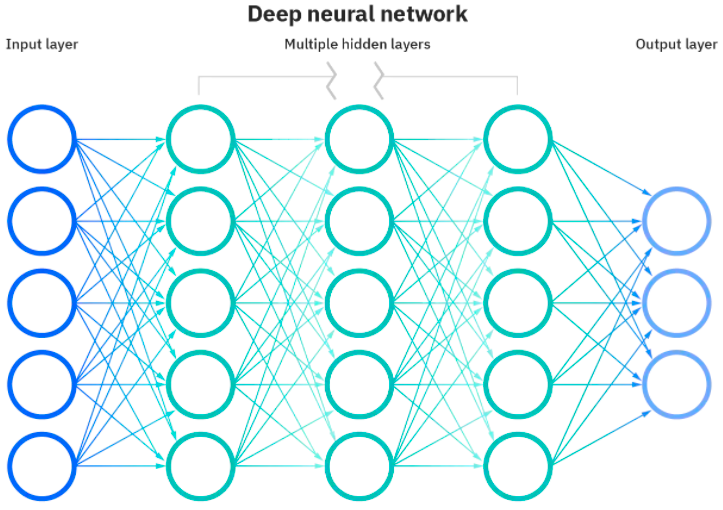
\includegraphics[width=0.7\textwidth]{figures/NN}
	\caption{A figure showing the layers of a Neural Network (see IBM, 2020)}
	\label{firstfig}
\end{figure}\newline
Neural networks depend on training data to learn and improve their accuracy over time. However, once these learning algorithms are polished for accuracy, they become powerful tools in computer science and artificial intelligence, allowing us to classify and cluster data at a high speed (see IBM, 2020).
\newline\newline
Neural network is good for returns prediction as it can accommodate nonlinear interactions, and no distribution is assumed. However, just like historical simulation they require large data set (which is not always available) for training to perform excellently well.
%%%%%%%%%%%%%%%%%%%%%%%%%%%%%%%%%%%%%%%%%%%%%%%%%%%%%%%%%%%
%%%%%%%%%%%%%%%%%%%%%%%%%%%%%%%%%%%%%%%%%%%%%%%%%%%%%%%%%%%




%%%%%%%%%%%%%%%%%%%%%%%%%%%%%%%%%%%%%%%%%%%%%%%%%%%%%%%%%%%
%%%%%%%%%%%%%%%%%%%%%%%%%%%%%%%%%%%%%%%%%%%%%%%%%%%%%%%%%%%

\section{Mathematics of Neural Network}
The main idea as well as the figures of this section is gotten from the thesis of Chaoyi Lou, titled Artificial Neural Networks:
their Training Process and Applications.
%%%%%%%%%%%%%%%%%%%%%%%%%%%%%%%%%%%%%%%%%%%%%%%%%%%%%%%%%%%
%%%%%%%%%%%%%%%%%%%%%%%%%%%%%%%%%%%%%%%%%%%%%%%%%%%%%%%%%%%

\subsection{A single Neuron}
\begin{figure}[!h]
	\centering
	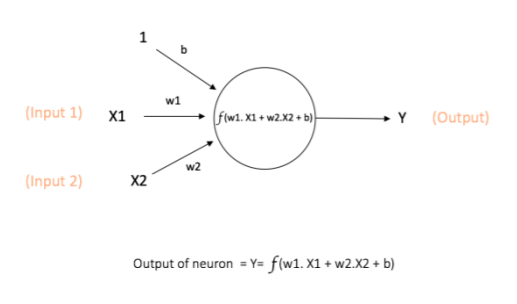
\includegraphics[width=0.7\textwidth]{figures/neuron}
	\caption{A single neuron of neural networks}
	\label{secondfig}
\end{figure}

\autoref{secondfig} shows a network with one layer containing a single neuron. This neuron receives input from the prior input layer, performs computations, and gives output. $x_1$ and $x_2$ are inputs with weights $w_1$ and $w_2$ respectively. The neuron applies a function $f$ to the dot-product of these inputs, which is $w_{1}x{1}+w_{2}x_{2}+b$.  Aside these two numerical input values, there is one input value 1 with weight $b$, called the Bias. The main function of bias is to represent unknown parameters. The dot-product of all input values and their associated weights is fed into the function $f$ to produce the result $Y$.
This function is known as Activation Function.\newline\newline
Activation functions are needed because many problems take multiple influencing factors into account and yield classifications. When faced with a binary classification problem, where the outcomes are either yes or no, activation functions are required to map the outcomes within this range. If a problem involving probability arises, one would expect the neural network's predictions to fall within the range of [0, 1]. This is what activation functions can do.\newline\newline
Linear and non-linear activation functions are the two types of activation functions. The most significant disadvantage of linear ones is that they cannot learn complex function mappings because they are only one-degree polynomials. As a result, non-linear activation functions are always required to produce results in desirable ranges and deliver them as inputs to the next layer. Few of the generally used non-linear activation functions will be discussed in the next section.
\subsection{Activation Functions}
An activation function takes the previously specified dot-product as an input and makes computation with it. Based on the range of the expected result, we place a certain activation function inside hidden layer neurons. The fact that activation functions should be differentiable is important because we'll use it later to train the neural network using backpropagation optimization.
\newline\newline
Here are few commonly used activation functions:\newline\newline
\textbf{Sigmoid}: This takes a real-valued input and returns a output in the range [0,1]:\newline\newline
$\delta = \frac{1}{1+e^{-x}}$
\begin{figure}[!h]
	\centering
	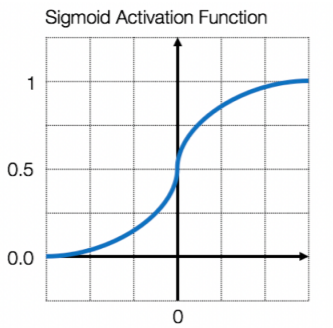
\includegraphics[width=0.4\textwidth]{figures/neuro}
	\caption{Sigmoid() Activation Function}
	\label{thirdfig}
\end{figure}

\autoref{thirdfig} shows an S-shaped curve and the values going
through the Sigmoid function will be within the range of [0, 1].
As the sigmoid function attains all values between 0 and 1 (with 0 and 1 attained in the limiting cases), the sigmoid function (also called logistic function) is a compatible probability transfer function.
Despite the fact that the Sigmoid function is simple to comprehend and use, it is not widely used due to its vanishing gradient problem. The issue is that the gradient can come so close to zero in some circumstances that it fails to properly adjust the weight. In the worst-case scenario, the neural network's ability to learn will be completely disabled. Second, this function's output is not zero-centered, causing gradient updates to travel in many different directions. Furthermore, the fact that the output is limited to the range [0, 1] makes optimization more difficult.
In order to compensate the deficiencies, tanh() is an alternative option
because it is a stretched version of the Sigmoid function with zero-centered outputs. \newline\newline
\textbf{tanh}: This takes real-valued input and produces the results in the range [-1, 1]:\newline\newline
$\text{tanh(x)}=\frac{sinh(x)}{cosh(x)}=\frac{e^{x}-e^{-x}}{e^{x}+e^{-x}}$

\begin{figure}[!h]
	\centering
	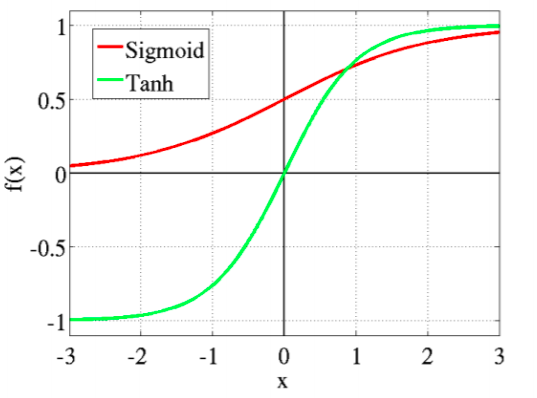
\includegraphics[width=0.4\textwidth]{figures/tanh}
	\caption{tanh() Activation Function}
	\label{fourthfig}
\end{figure}

The benefit of this function is that negative input values will be mapped strongly negative, and extremely small values close to zero will be mapped to values close to zero. As a result, this function is helpful in doing a classification between two classes.
Though in reality, this function is favoured over the Sigmoid function (because of the greater output range), the gradient vanishing problem still occurs. Using a reasonably simple formula, the following ReLU function corrects this problem.\newline\newline
\textbf{ReLU} (Rectified Linear Unit): ReLU is just another name for the positive part of the argument, i.e it takes a real-valued input and replaces the negative values with zero:
\newline\newline
$R(x)= \text{max}(0,x)$
\begin{figure}[!h]
	\centering
	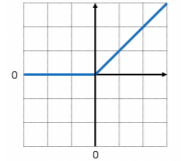
\includegraphics[width=0.4\textwidth]{figures/Relu}
	\caption{ReLU() Activation Function}
	\label{fifthfig}
\end{figure}
\newline\newline As it is a very simple and efficient function that avoids and corrects the gradient vanishing problem, it is employed in practically all convolutional neural networks or deep learning.
The difficulty with this activation function is that after it is activated, all negative values become zeros, which has an impact on the outcomes because negative values are not taken into account.
\newline\newline When we know what qualities of outcomes we want to observe, we apply different activation functions.
 \section{General Model Building}
 Having discussed the mathematics behind neural network, it is however important to talk about the neural network architectures and other components
 \subsection{Neural network Architures}
 Neural Networks are complex structures made of artificial neurons that can accommodate several inputs to produce output(s). As stated earlier, a neural network consists of an input layer, one or multiple hidden layers and output layer(s). In a dense neural network, all the neurons (contained in each layers) affect each other, and hence, they are all connected. How the input neurons produce a certain output depends
 on the structure of the neural network. The two main classes of network architectures are discussed below
 \subsubsection{Feed-forward Neural Network} (see Bijelic \& Ouijjane, 2019)
 In feed-forward neural network(FFN), each neuron in a
 particular layer is connected with all neurons in a subsequent layer. The information
 flow in the network is of feedforward type (i.e the connections
 can never skip a layer, or form any loops backwards).
 \newpage
 \begin{figure}
 	\centering
 	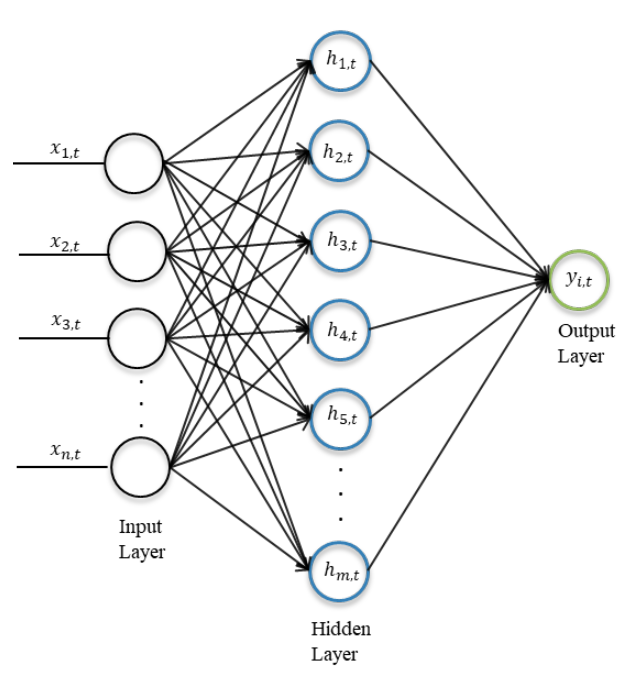
\includegraphics[width=0.4\textwidth]{figures/FFN}
 	\caption{A fully connected FFN with a single hidden layer (see Bijelic \& Ouijjane, 2019)}
 		\label{sixthfig}
 \end{figure}
 As shown in the above figure, the values of the input are transported to the hidden layer through connections, each being characterised by certain weight coefficient, $W_{i,k}$. The degree of connection between the input node and a hidden node is reflected by these weight coefficients. Defining [$x_{1,t};x_{2,t};...;x_{n,t}$] as the vector of the input signals and [$h_{1,t};h_{2,t};...;h_{m,t}$], the propagation of the input nodes to one hidden node can
 mathematically be described by: 
 \begin{center}


 $h_{k,t} =\sum_{i=1}^{n} W_{i,k} \cdot x_{i,t}$ for $k = 1,2,...,m$
  \end{center}
An undesirable property of the formula is its linear representation,
which, if applied, would suggest that the output prediction would be a linear function, which is not always the case. In order to deal with this, a non-linear activation function, $\Phi(\cdot)$ is applied to the weighted sum of
inputs into a hidden node. This activation function, which in the majority of
applications takes the form of a sigmoid function or a ReLu function, makes the neural network a universal approximator i.e neural networks have the capability of approximating
any measurable function to any desired degree
of accuracy, in a very specific and satisfying
sense (see Hornik et al (1989) for details). However, before applying
the activation function, a bias vector [$b_{1};b_{2};...;b_{m}$] is added, which essentially
indicates whether a neuron tends to be active or inactive in the prediction process. The
propagation from the input layer to the hidden layer in a feed-forward neural
network may now be reformulated to:
 \begin{center}
	$h_{k,t} =\Phi(b_{k,0} +\sum_{i=1}^{n} W_{i,k} \cdot x_{i,t}$) for $k = 1,2,...,m$
\end{center}
The feedforward neural network has the major disadvantage that it cannot model temporal dependencies in the data. However, this shortcoming of not being able to account for correlations between inputs is overcome in the recurrent neural network, which is able to selectively feed forward information over sequences of elements by generating cycles in the network.
\subsubsection{Recurrent Neural Network} (see Bijelic \& Ouijjane, 2019)
Recurrent Neural Networks
(RNN) can handle sequential data due to the capability of each neuron to
maintain information about previous inputs, contrary feedforward neural networks. This implies that the prediction a recurrent
neural network node made at previous time step $t-1$ affects the prediction it will make one
moment later, at time step $t$. RNN nodes can be thought of as having memory as it takes inputs not only the current signal, but also
what has been perceived previously in time.\newline\newline
RNNs contain feedback loops from the so-called hidden states, and this allows preservation of information from one node to another while reading in inputs. At each time step in the data series, the feedback loop mechanism occurs, which causes each hidden state to contain traces not only of the respective hidden state before it, but also of all those preceding it, for as long as the memory of the network lasts.\newline
\begin{figure}[h]
	\centering
	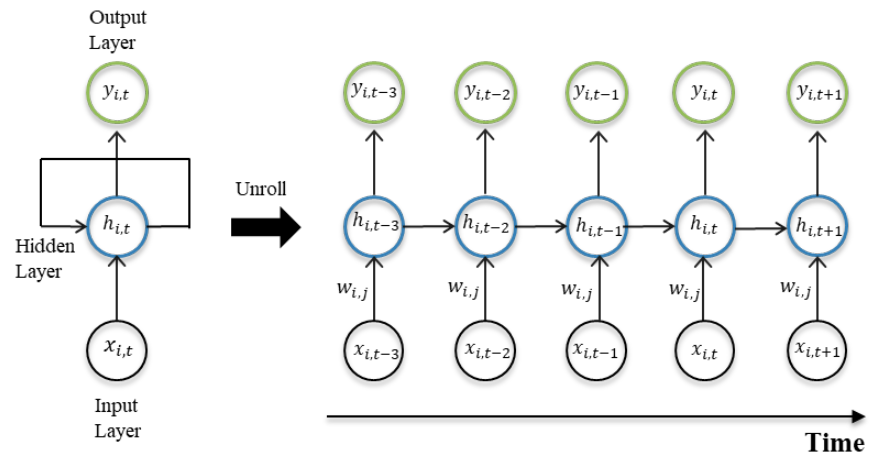
\includegraphics[width=0.4\textwidth]{figures/RNN}
	\caption{Representation of an unrolled plain vanilla recurrent neural network. (see Bijelic \& Ouijjane, 2019)}
	
	\label{seventhfig}
\end{figure}

The unrolled RNN shows how the network enables the hidden neurons to see their
own previous output, so that their subsequent behavior can be shaped by their responses in the past (Tenti, 1996). In addition, utilization of a RNN is particularly desired when there are
time dependencies in the data series, this is evident when we introduce time-lagged model components. Using the initial notation, and suppose that the hidden states are the ones looped
back, the output from a hidden node in the RNN model relies not only on the input values at
time $t$, but also on its own lagged values at order $p$ as represented below:

\begin{center}
	$h_{k,t} =\Phi(b_{k,0} + \sum_{i=1}^{n} W_{i,k} \cdot x_{i,t}) + \sum_{k=1}^{m} \gamma_{k} \cdot h_{k,t-p}$for $k = 1,2,...,m$
\end{center}

where $h_{k,t-p}$ represents the lagged hidden state values at order $p$, and $\gamma_{k}$ a coefficient. Another outstanding feature of recurrent networks is that recurrent neural networks share the same weight parameter within each layer of the network, unlike feedforward networks that have different weights across each node. Through the processes of backpropagation and gradient descent these weights are adjusted to enable reinforcement learning.  Backpropagation through time (BPTT) algorithm is exploited by Recurrent neural networks to determine the gradients, which is a bit different from traditional backpropagation as it is specific to sequence data. In BPTT errors are summed up at each time step whereas feedforward networks do not have to sum errors because it shares no parameter across each layer (see IBM 2020 for details).\newline\newline
In this process, RNNs tend to experience two issues, known as exploding gradients and vanishing gradients. These issues are defined by the gradient size, which is the slope of the loss function along the error curve. If the gradient is too small, the weight parameters will be updated until they become insignificant - i.e. 0, and the algorithm will no longer learn. Gradients explode when they are too large, creating an unstable model. In this case, the model weights will grow too large and will eventually be labelled NaN values. In order to reduce these issues, it is possible to reduce the number of hidden layers within the neural network, thereby reducing its complexity (see IBM 2020).

\subsubsection{Long Short-Term Memory Recurrent Neural Network}
LSTM is a class of recurrent neural networks and its main feature is its purpose-built memory cells, which allows it to capture long range dependencies in the data.\newline\newline
A previous sequence element and the output from the network function serve as input for the next sequence element in the network function. As such, the LSTM can be compared to a HMM (Hidden Markov Model), in which there is a hidden state which conditions the output distribution. Furthermore, LSTM hidden state not only depends on its previous states but also reflects long-term sequence dependence since it is recurrent. In particular, the receptive field size of an LSTM (i.e. the size of the input region that generates the feature) is unbounded architecture-wise, unlike simple feed forward networks and CNNs (see Arimond et al, 2020). Due to the attractiveness of the LSTM, it will be used in this work to forecast volatility of returns of stock markets. 

\begin{figure}[h]
	\centering
	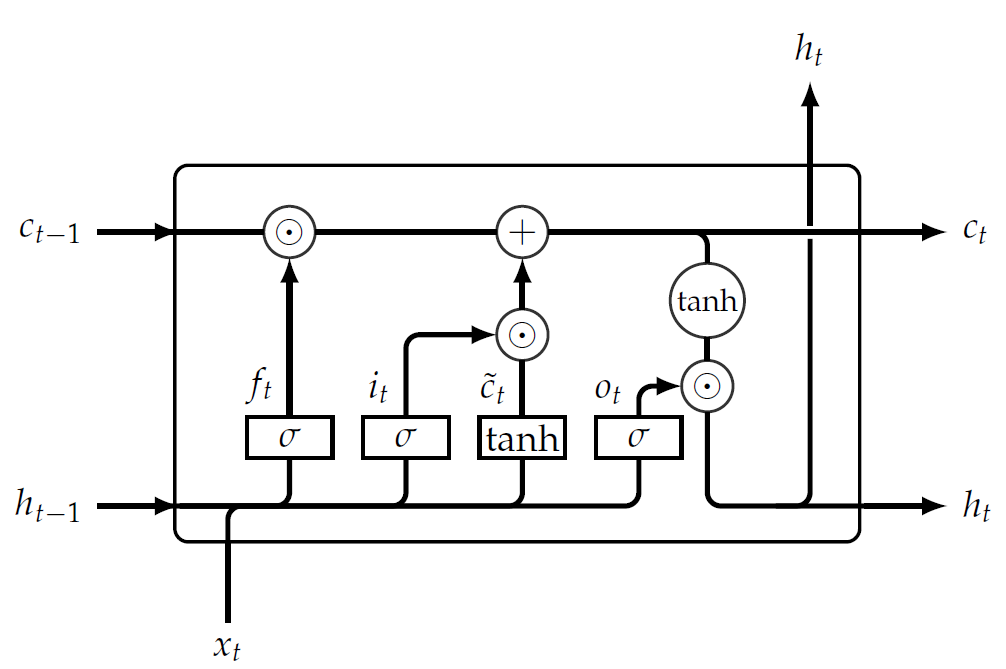
\includegraphics[width=0.4\textwidth]{figures/lstm}
	\caption{Diagrammatic representation of an LSTM cell  (see KRETSCHMER, 2019)}
	
	\label{lstm}
\end{figure}

LSTM has basically the same setting as the standard RNN. In each time step $t$, the input $x_t$ and the past state information, for an LSTM $c_{t-1}$ and $h_{t-1}$, are taken into the hidden mapping. However, in the LSTM the hidden mapping is not just a linear layer followed by an activation function. It rather uses a group of gates and activations to determine the flow of information. A representation of the architecture is shown in the above figure where the rectangular blocks represent layers and nodes pointwise operations.\newline\newline
A gate is a simple sigmoid layer which may at its extremes be either open or closed if its outputs 1 or 0 respectively, depending on the input. For this reason, if another variable gets multiplied by such a gate, the model may either pass the variables information (gate open) or ends the flow (gate closed). The forget, the input and the output gate exist in LSTM\\\\
In contradiction to the basic RNN, the LSTM has two state variables: the cell state and the hidden state. The cell state may be seen as a summary statistic of past and current  information and the hidden state may be viewed as a polished version of the cell state capturing enough information for the output.\\\\
Let us have a look at each of the steps within an LSTM cell

\begin{description}
	\item[$\bullet$] Forget\\
	First, the LSTM determines which part of the past information in the cell state $c_{t-1}$ can be removed. This may be useful if context changes and previous information is no longer a valid predictor for future tasks. Hence, the forget gate $f_t$ is calculated based on the  past hidden state $h_{t-1}$ and the current input $x_t$
\begin{center}
	$f_t$ =  $\sigma(W_{f}x_{t}+V_{f}h_{t-1}+b_{f})\in (0,1)^{D}$
\end{center}
\item[$\bullet$] Input\\
Next, the LSTM recognizes new information which should be incorporated in the cell state $c_t$. Like the forget gate, the input gate $i_t$ gets calculated
\begin{center}
	$i_t$ =  $\sigma(W_{i}x_{t}+V_{i}h_{t-1}+b_{i})\in (0,1)^{D}$
\end{center}
to decide which part of the cell state to add the new information $\tilde{c_t}$ given by 
\begin{center}
	$\tilde{c_t}$ =  $\text{tanh}(W_{c}x_{t}+V_{c}h_{t-1}+b_{c})\in (-1,1)^{D}$
\end{center}

\item[$\bullet$] Update cell state\\
Combine Step 1 and Step 2 to obtain the new cell state

\begin{center}
	${c_t}$ =  $f_{t} \odot c_{t-1}+i_{t}\odot \tilde{c_t} \in \mathbb{R}^{D}$
\end{center}
giving a summary statistics of relevant past and current information. "$\odot$" represents Hadamard product which is the element-wise multiplication of matrices.

\item[$\bullet$] Update hidden state\\
Determine the parts of the cell state that are enough for the output by calculating
the output gate
\begin{center}
	$o_t$ =  $\sigma(W_{o}x_{t}+V_{o}h_{t-1}+b_{o})\in (0,1)^{D}$
\end{center}
and use this to determine the hidden state $h_t$ as a polished version of the cell state.

\begin{center}
	$h_t$ =  $o_t \odot \text{tanh}(c_t)\in (-1,1)^{D}$
\end{center}

\end{description}
(see KRETSCHMER, 2019)









\section{The LSTM Architecture}
Our LSTM has a single hidden layer,  with 'tanh' as the activation function. The following are the parameters (all but MSE has to be determined before you can actually start training, validating and testing your LSTM net) used in within the LSTM neural network:
\begin{itemize}

\item[$\bullet$]   
To determine the best weights of the neural network, Adam (Adaptive Moment Estimation) is the chosen optimizer in our LSTM model. Some of its advantages are that the sizes of parameter updates are invariant to
rescaling of the gradient, its stepsizes are approximately bounded by the stepsize hyperparameter, stationary objective is not required, it works with sparse gradients, and it naturally performs a
form of step size annealing (see Kingma and Ba, 2015).
\item[$\bullet$] The batch size is the number of inputs that will be propagated in the
LSTM neural network during the training process. In our LSTM model 128 is the chosen batch size, and this means that the inputs are
fed in the network in batches, each containing 128 inputs. After
the propagation of a batch, the network is trained before receiving another
batch of 128 inputs. This operation continues until all inputs are propagated.
\item[$\bullet$] The look ahead is the amount of time steps, i.e. the lagged
inputs the RNN should use to forecast the desired outputs. For all trials, the look ahead is set to 90 lagged inputs, which
corresponds to about 3-month period in the data sample.
\item[$\bullet$] The dropout function is a regularization method used to prevent overfitting by
allowing the LSTM neural network to drop a random set of neurons while
training the network. Ignoring several neurons for each iteration during the
training process is necessary, because if the network is fully connected,
neurons will become interdependent, leading to overfitting of the training data. For example, if the dropout function is set to 0.25, this means that 25\% of the existing
neurons within the network will be ignored during the training process (in different training steps one drops different neurons as otherwise you will not train the full network).
\item[$\bullet$] The number of epochs can also influence the accuracy of a neural network. It
refers to the number of times all the training and validation datasets are
propagated through the LSTM neural network. The standard procedure is to
increase the number of epochs until the chosen metric – in this case the MSE
– decreases for the validation set, while it continues to increase for the training
set, i.e. when the training set shows signs of overfitting.
\item[$\bullet$] The Mean Square Error (MSE): This is the average squared difference between the estimated values and the actual value.
\end{itemize}

\begin{center}
	$L_{MSE} = 1/N\sum_{k=1}^{N} ({\hat{y}}_{k}-y_k)^2$
\end{center}
It is also chosen as the loss function (between the predicted outputs and the actual outputs) and the performance measure(to assess the model fit while
training and validating the network) of the
LSTM neural network.\\\\
The number of neurons, dropout function, and epochs are changed in each LSTM models to choose the one that performs best. That is, the LSTM with the lowest MSE value. This will be discussed in details in the next chapter.


%%%%%%%%%%%%%%%%%%%%%%%%%%%%%%%%%%%%%%%%%%%%%%%%%%%%%%%%%%%
%%%%%%%%%%%%%%%%%%%%%%%%%%%%%%%%%%%%%%%%%%%%%%%%%%%%%%%%%%%
%%%%%%%%%%%%%%%%%%%%%%%%%%%%%%%%%%%%%%%%%%%%%%%%%%%%%%%%%%%
\chapter{Numerical comparisons}
For the empirical study, the day-ahead forecasting of the 1\% and 5\% VAR for daily log-returns(natural log of the new value divided by the initial value) of the following stock markets: NIKKEI 225, FTSE 100 and S\&P 500 are considered. The data is downloaded from DataStream. Each series (NIKKEI 225, FTSE 100 and S\&P 500) consist of 8477 daily price indices (measure of how prices change over a period of time), the start date and end date are 04/01/1988 and 30/06/2020 respectively. Upon calculating the log-returns, which is given as 

\begin{center}
	$R_t = ln(\frac{S_t}{S_{t-1}})$, where ${S_t}$ and ${S_{t-1}}$ are current return and initial return respectively
\end{center}
the data in the first row of the series vanishes leaving us with 8476 daily log-returns and 05/01/1988 as starting date. Basically, this means we use 8476 daily log-returns for our VaR estimation. This longer sample is desirable for our models, most especially the historical simulation and neural network as they work best with large data. Moreover, data contains periods of low and high volatilities, which mitigates the probability of the historical simulation being bias (underestimation or overestimation) in the return estimation.\newline

\begin{figure}[!h]
	\centering
	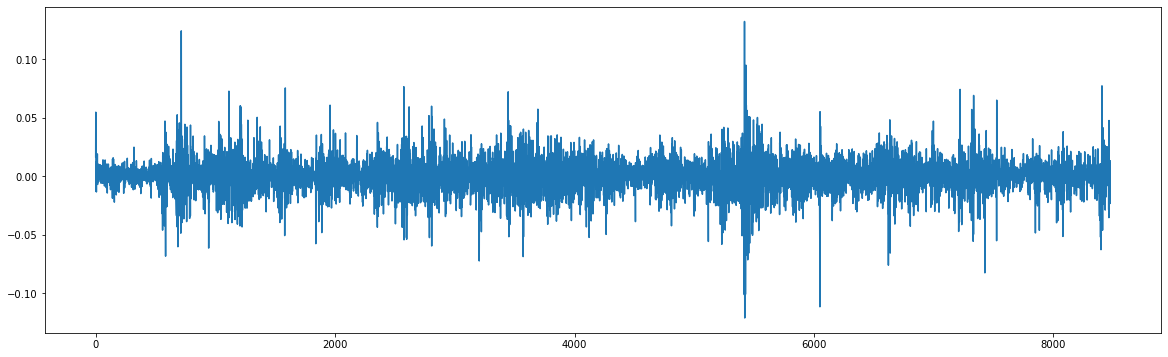
\includegraphics[width=0.8\textwidth]{figures/logNikkei}
	\caption{The series of log-returns of Nikkei 225}
	\label{logNikkei}
\end{figure}

\begin{figure}[!h]
	\centering
	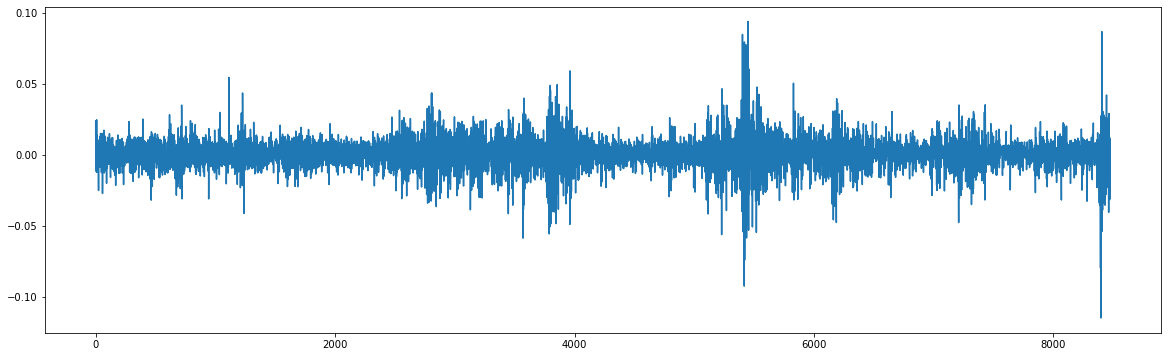
\includegraphics[width=0.8\textwidth]{figures/logFTSE}
	\caption{The series of log-returns of FTSE 100}
	\label{logFTSE}
\end{figure}


\begin{figure}[!h]
	\centering
	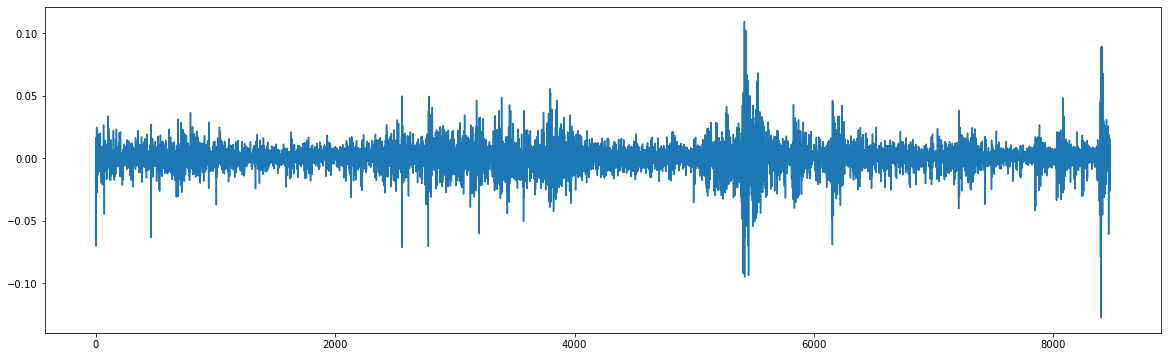
\includegraphics[width=0.8\textwidth]{figures/logS&P500}
	\caption{The series of log-returns of S\&P 500}
	\label{logSandP 500}
\end{figure}

\section{Partitioning the Dataset}
\subsection{LSTM Neural Network Model}

Our LSTM is used for time series predictions and our predictions will then be modelled into VaR estimates. Generally, data is divided into two main parts in neural network models: training set and test set. However, an additional intermediate set called validation set (sometimes modelled as part of training), is sometimes employed in order to avoid overfitting. The training and validation data can be jointly referred to as In-sample data, while the test data is sometimes referred to as Out-of-sample data. In most literatures, the common choice for training set between 70\% to 90\% of the original dataset, and 10\% to 20\% of the training are used as validation dataset. The rest are, of course the testing dataset, which will be to evaluate our predictions using MSE and also compared with our value at risk estimates. \newline\newline
In this study, we have a lookahead (timestep) of 90 days, and in turn, we are left with 8386 days for training and testing. The first 7000 daily log-returns of each series are used as training dataset, which is around 83\% of each of the series. The last 1400 (20\%) values (daily log-returns) of the training dataset are used for validation. The remaining 1386 daily log-returns are used for testing. The dates for the data split are reported in the table below.
%\makeatletter
%\setlength\@fptop{0\p@}
%\makeatother
\newline\newline
\begin{table}[!h]
	\centering
	\begin{tabular}{l|cl}
		\hline \hline
		In-sample
		& out-of-sample\\ \hline
		Training set: 10/05/1988 – 26/10/2009
		& Test set
		: 10/03/2015 – 30/06/2020
	 \\
		Validation set: 27/10/2009– 09/03/2015
		\\
		\hline \hline
	\end{tabular}
	\caption{Data splits}
	%\vspace{128in}
	\label{firsttab}
\end{table}

An important pre-processing step is input normalization, as it is considered good practice for neural network training, data scaling helps neural networks train and converge faster. We use the z-score (StandardScaler): 

\begin{center}
	$X_{new} = \frac{X_{i}-\mu}{\sigma}$
\end{center}

where $X_{new}$ is the standardized data point, $X_{i}$ is the initial data point, $\mu$ is the sample mean and $\sigma$ is the sample standard deviation.


\subsection{Historical simulation and GARCH(1,1) Volatility model}
For congruency with the LSTM model (in regards to number of predictions), we use a rolling window of 7090 for Historical simulation and GARCH(1,1) Volatility model, which stands as our in-sample data and we have 1386 out-of-sample data.

\subsection{Trial Results of the LSTM Neural Network}

As discussed in the previous chapter, the performance of our LSTM model is based on MSE. In this paper, we follow a best-out-of-5 approach, that means for each stock market, we train our model five times with different values of the parameters and the best one (in each of the model training for the three stock market) is selected for VAR estimation. Tanh is the activation function in all models.\newline\newline
\textbf{NIKKEI}


\begin{center}
	\begin{tabular}{||c c c c c||} 
		\hline
		Trials & Epochs & Dropout & Hidden Neurons & Validation result\\ [0.5ex] 
		\hline\hline
		1 & 500 & 0.1 & 100 & 0.0002802554 \\ 
		\hline
		2 & 190 & 0.1 & 100 & 0.00020421705 \\
		\hline
		3 & 111 & 0.2 & 100 & 0.0001736877 \\
		\hline
		4 & 111 & 0.2 & 150 & 0.0001814346 \\
		\hline
		5 & 111 & 0.3 & 150 & 0.0001725089\\ [1ex] 
		\hline
	\end{tabular}
\end{center}

In the first trial, the model is trained for 500 epochs. Both training and validation losses keep reducing until around 120 epochs where model begins to show overfitting as validation loss starts increasing. Overfitting becomes obvious after 190 epochs.\newline
\begin{figure}[!h]
	\centering
	\includegraphics[width=0.8\textwidth]{figures/Nik1}
	\caption{Training and Validation loss functions under Trial 1 (Nikkei 225))}
	\label{Nik1}
\end{figure}


 The second test is run with 190 epochs to discard the utmost overfitting and to confirm the intuition that the lowest loss on the validation set exists
 before the 120th epoch. Here the validation loss has its lowest value at 111th epoch. 
\begin{figure}[!h]
	\centering
	\includegraphics[width=0.8\textwidth]{figures/Nik2}
	\caption{Training and Validation loss functions under Trial 2 (Nikkei 225))}
	\label{Nik2}
\end{figure}

As the perfect amount of epochs has been known, we run our third trial with 111 epochs and we increase our dropout. This model has the second lowest MSE. 
\newpage
\begin{figure}[!h]
	\centering
	\includegraphics[width=0.8\textwidth]{figures/Nik3}
	\caption{Training and Validation loss functions under Trial 3 (Nikkei 225))}
	\label{Nik3}
\end{figure}
We perform our fourth model with an increase in the amount of neurons in the hidden layer to see if our model will perform better, but this is not the case as it has a higher MSE than the third model.
\newline
\begin{figure}[!h]
	\centering
	\includegraphics[width=0.8\textwidth]{figures/Nik4}
	\caption{Training and Validation loss functions under Trial 4 (Nikkei 225))}
	\label{Nik4}
\end{figure}

The best performed model is the fifth trial. We maintain 150 neurons in the hidden layer, however we increase the amount of dropout to 0.3. This model will be chosen for our VaR estimation.\newline
\begin{figure}[!h]
	\centering
	\includegraphics[width=0.8\textwidth]{figures/Nik5}
	\caption{Training and Validation loss functions under Trial 5 (Nikkei 225))}
	\label{Nik5}
\end{figure}
\newline\textbf{FTSE 100}


\begin{center}
	\begin{tabular}{||c c c c c||} 
		\hline
		Trials & Epochs & Dropout & Hidden Neurons & Validation result\\ [0.5ex] 
		\hline\hline
		1 & 500 & 0.1 & 100 & 0.00018413635 \\ 
		\hline
		2 & 200 & 0.1 & 100 & 0.00013991451 \\
		\hline
		3 & 147 & 0.1 & 120 & 0.00013827156 \\
		\hline
		4 & 147 & 0.2 & 120 & 0.00013800853 \\
		\hline
		5 & 147 & 0.3 & 100 & 0.00012749673\\ [1ex] 
		\hline
	\end{tabular}
\end{center}

In the first trial, the model is trained with 500 epochs. Both training and validation losses keep reducing until around 175 epochs where model begins to show overfitting as validation loss starts increasing. Overfitting becomes obvious after 200 epochs.

\begin{figure}[!h]
	\centering
	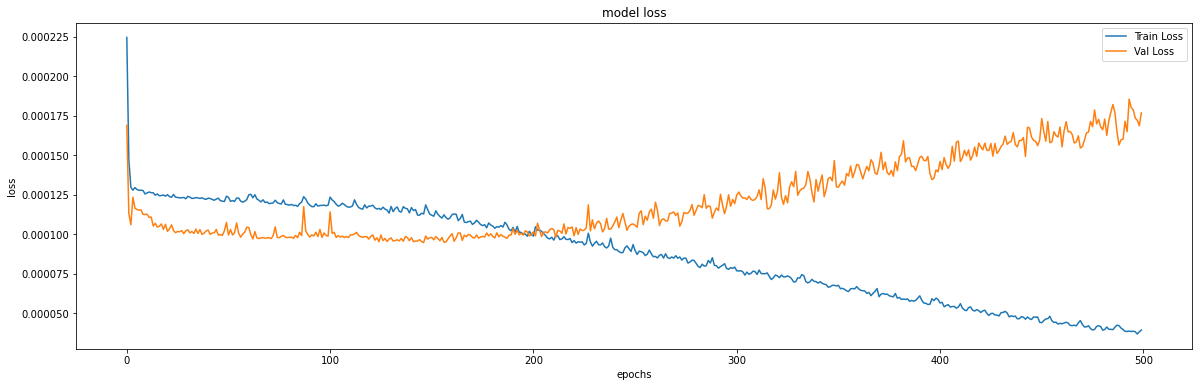
\includegraphics[width=0.8\textwidth]{figures/FTSE1}
	\caption{Training and Validation loss functions under Trial 1 (FTSE 100))}
	\label{FTSE1}
\end{figure}
 The second trial of our lstm model is trained with 200 epochs to remove the obvious overfitting. Here it becomes clear that our model performs well till 147 epochs after which validation losses continue to increase. 
\begin{figure}[!h]
	\centering
	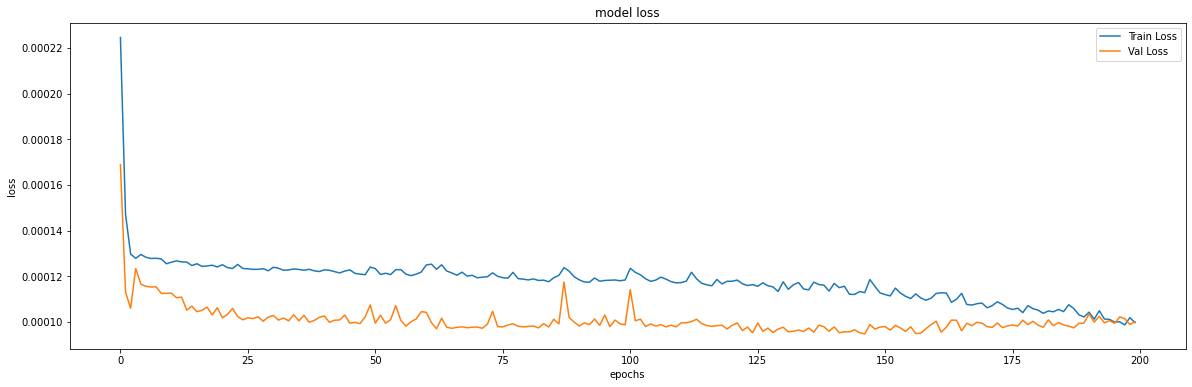
\includegraphics[width=0.8\textwidth]{figures/FTSE2}
	\caption{Training and Validation loss functions under Trial 2 (FTSE 100))}
	\label{FTSE2}
\end{figure}

 We perform the third trial with the required 147 epochs and the amount of neurons in the hidden layers is increased to 120. This model gives the third lowest MSE.

\begin{figure}[!h]
	\centering
	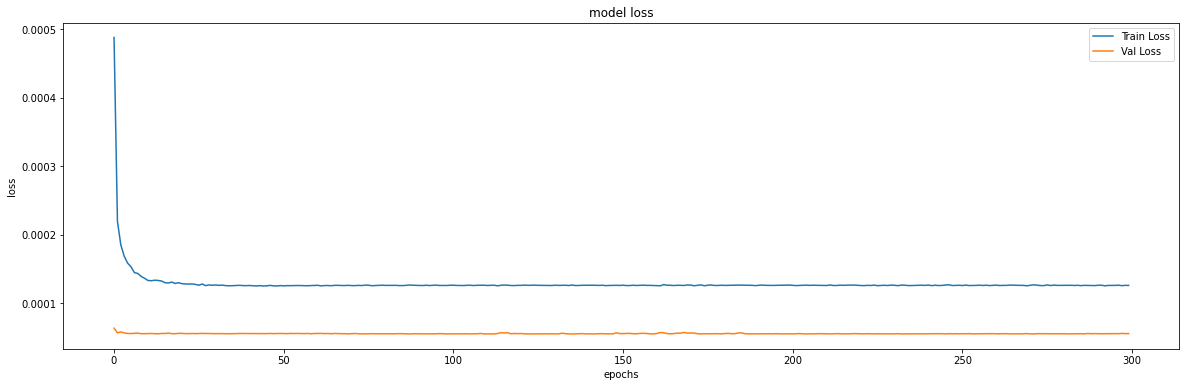
\includegraphics[width=0.8\textwidth]{figures/FTSE3}
	\caption{Training and Validation loss functions under Trial 3 (FTSE 100))}
	\label{FTSE3}
\end{figure}
 The fourth trial is trained with 147 epochs, the increased amount of dropout leads to a lower MSE result compared to the third trial. 
 \newpage

\begin{figure}[!h]
	\centering
	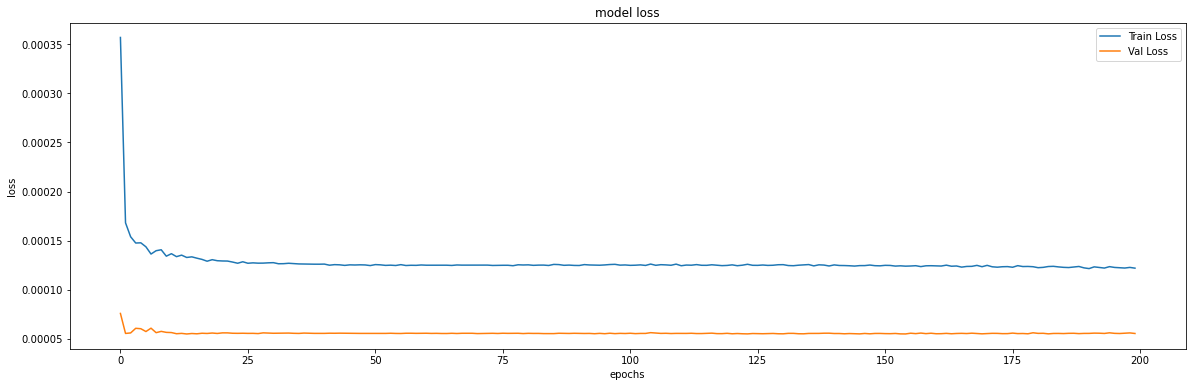
\includegraphics[width=0.8\textwidth]{figures/FTSE4}
	\caption{Training and Validation loss functions under Trial 4 (FTSE 100))}
	\label{FTSE4}
\end{figure}

 The last trial is the chosen model for our VaR estimation as it performs best. Dropout is increased while we reduce the amount of neurons in the hidden layer. 
\begin{figure}[!h]
	\centering
	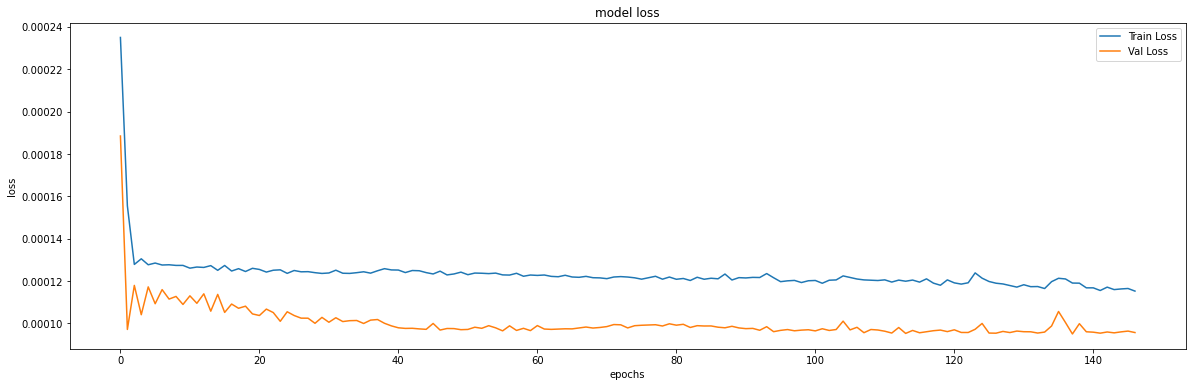
\includegraphics[width=0.8\textwidth]{figures/FTSE5}
	\caption{Training and Validation loss functions under Trial 5 (FTSE 100))}
	\label{FTSE5}
\end{figure}
 
 
 \textbf{S\&P500}


\begin{center}
	\begin{tabular}{||c c c c c||} 
		\hline
		Trials & Epochs & Dropout & Hidden Neurons & Validation result\\ [0.5ex] 
		\hline\hline
		1 & 500 & 0.1 & 100 & 0.00023379210 \\ 
		\hline
		2 & 195 & 0.2 & 100 & 0.00015249624 \\
		\hline
		3 & 124 & 0.2 & 120 & 0.00014183349 \\
		\hline
		4 & 124 & 0.2 & 180 & 0.00014573926 \\
		\hline
		5 & 124 & 0.3 & 180 & 0.00015285780 \\ [1ex] 
		\hline
	\end{tabular}
\end{center}

In the first trial, the model is trained with 500 epochs. Both training and validation losses keep reducing until around 150 epochs where model begins to show overfitting as validation loss starts increasing. Overfitting becomes obvious after 195 epochs.\newline
\begin{figure}[!h]
	\centering
	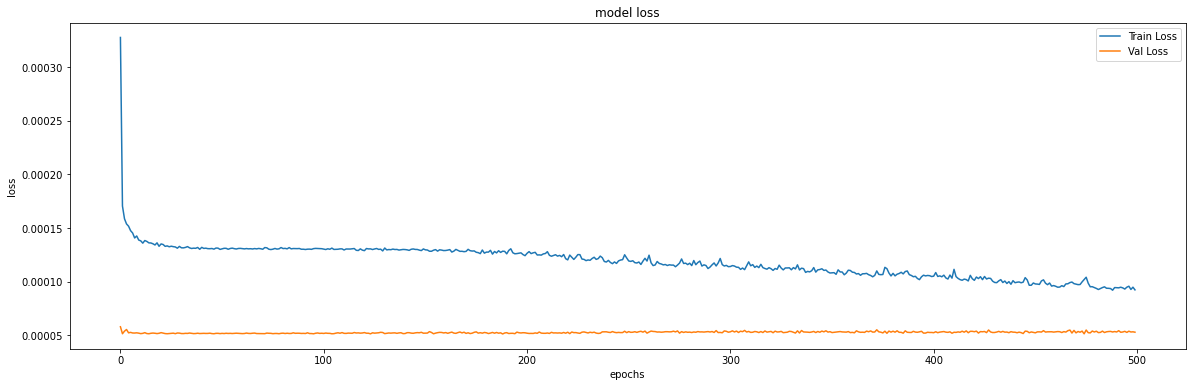
\includegraphics[width=0.8\textwidth]{figures/sanp1}
	\caption{Training and Validation loss functions under Trial 1 (S\&P 500)}
	\label{sanp1}
\end{figure}
\newline The second test is run with 195 epochs to discard the utmost overfitting and to confirm the intuition that the lowest loss on the validation set exists
before the 150th epoch. It becomes clear that our model performs well till 147 epochs after which validation losses keeps increasing.  
\begin{figure}[!h]
	\centering
	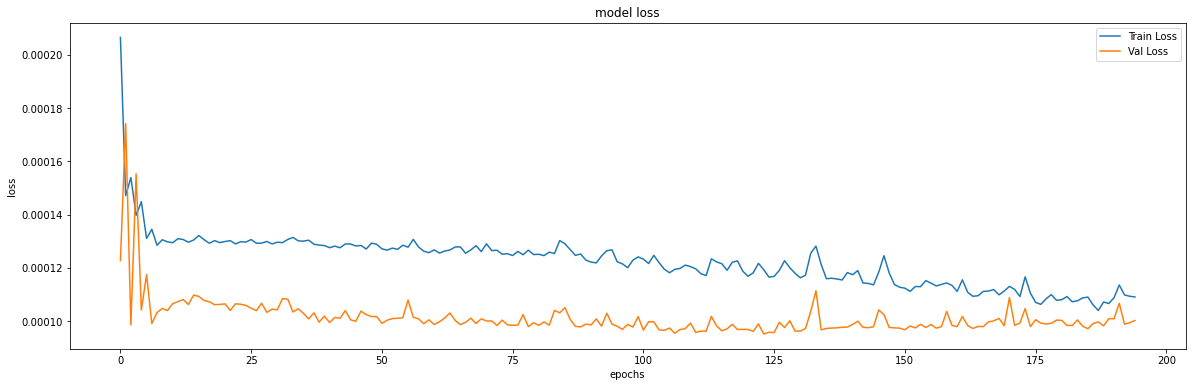
\includegraphics[width=0.8\textwidth]{figures/sanp2}
	\caption{Training and Validation loss functions under Trial 2 (S\&P 500)}
	\label{sanp2}
\end{figure}
 We perform the third trial with the required 124 epochs and the amount of neurons in the hidden layers is increased to 120. This model gives the lowest MSE and will be used for VaR estimation.\newline
\begin{figure}[!h]
	\centering
	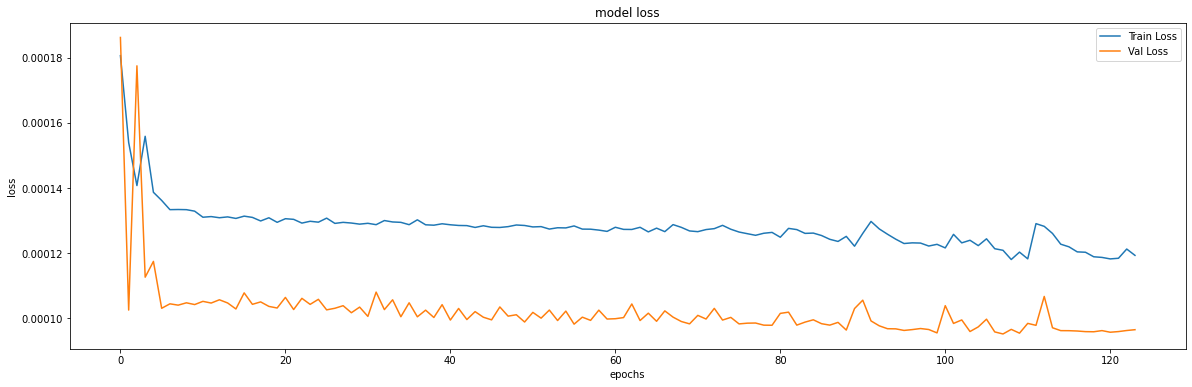
\includegraphics[width=0.8\textwidth]{figures/sanp3}
	\caption{Training and Validation loss functions under Trial 3 (S\&P 500)}
	\label{sanp3}
\end{figure}

The penultimate trial is trained with the sufficient 124 epochs. The increased amount of neurons without an increase in the dropout seems to alter its performance \newline
\begin{figure}[!h]
	\centering
	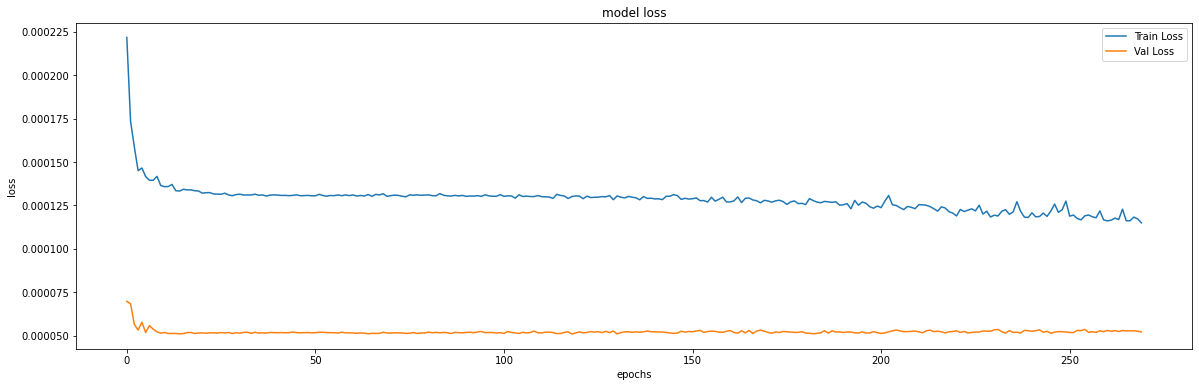
\includegraphics[width=0.8\textwidth]{figures/sanp4}
	\caption{Training and Validation loss functions under Trial 4 (S\&P 500)}
	\label{sanp4}
\end{figure}
\newline The last trial is trained with the sufficient 124 epochs. Here we increase our dropout to 0.3 and this model takes the fourth position in terms of performance in respect to its MSE.
\begin{figure}[!h]
	\centering
	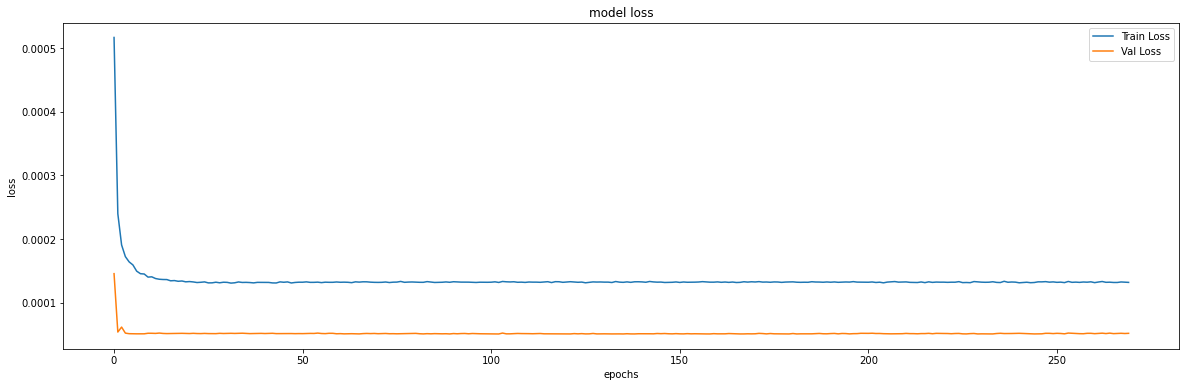
\includegraphics[width=0.8\textwidth]{figures/sanp5}
	\caption{Training and Validation loss functions under Trial 5 (S\&P 500)}
	\label{sanp5}
\end{figure}\newline\newline\newline\newline\newline

\section{VAR Estimation}
In this section, we discuss the estimation of our value at risk.
\subsection{Historical Simulation}
As a nonparametric method, we use historical simulation with rolling window of 7090 observations to estimate the value at risk for the next 1386 days.



\subsection{GARCH (1,1) model}

With a rolling window of 7090 observations, we estimate our daily VaR estimation of 1386 days using the conditional variance given by GARCH(1,1) model. We assume the random error to have a student’s t-distribution with 7089 degrees of freedom (calculated as N-1, where N= size of rolling window). Our Value at Risk is given by:
\begin{center}
$\text{VaR}_{t+1|t}$ = -$\mu_{t+1|t} - \sigma_{t+1|t} * q_{\alpha}$
\end{center}
where $\mu$ is the conditional mean, $\sigma$ is the conditional volatility, and $q_{\alpha}$ is the $\alpha$ quantile of the student's t-distribution.

\subsection{The LSTM model}
We determine our value at risk by calculating the 0.05 quantile (95\% Var) and 0.01 quantile (99\% Var) of our predicted values. The output generated by our LSTM model starts with the following form:
\begin{center}
	$y_1= tanh(\sum_{i=1}^{i=90}W_{i}u_{i}+\beta)+\varepsilon_t$
\end{center} 

where $u_{i}$ are the inputs, $W_i$ are the weights, $\beta$ is the bias and $\varepsilon_t$ = random error in the period $t$, which equals to the
product of standard deviation $\sigma_t$ of the calibration set and  the
standardized random error $\xi_t$ in the period $t$ ($\xi_t$ $\sim$ N(0,1)), tanh is the activation function. As the output from the network function serves as input for the next sequence element in the network function, the general equation of the output of the LSTM would be of the form:

\begin{center}
	$y_n= tanh(\sum_{i=1}^{i=90}W_{i}u_{i}+\sum_{i=1}^{n-1}y_{i}K_{i}+\beta)+\varepsilon_t$
\end{center} 
where $K_i$ are weights, $y_i$ are initial outputs.

\subsubsection{How we estimate our value at risk from our LSTM model}

Here we discuss the two approaches we use in estimating our VAR with LSTM model. 
\begin{itemize}
	
\item[$\bullet$]   We are at time $t$ and have given a trained NN that uses the (log-)returns of the last 90 days (up to
today) as input to predict the log return $r_{t+1}$ from time $t$ to time $t+1$.
\item[$\bullet$]      Now simulate 1000 predictions $r(1), ..., r(1000)$ of this log return from $t$ to $t+1$ by generating a standard normal distribution with a sample size of 1000, then scale these samples with the standard deviation of the historical returns (the first 7090 days of our original data that make up the timesteps and training). Then add each scaled samples to  our predicted return $r_{t+1}$. Call the ordered
predictions $p(1),p(2),...,p(1000)$.

\item[$\bullet$] Estimate the VaR95 = 0.5*($p(950)+p(951)$), VaR99 = 0.5*($p(990)+p(991)$)


\item[$\bullet$] Compare the actual log return $r_{t+1}$ in the test data set with VaR95 and VaR99 and increase the number
of breaches for VaR95 by 1 if you have VaR95 $<$ $r_{t+1}$ and do the same for VaR99.

\item[$\bullet$] Then update your trained NN by moving one time step forward, i.e. by including the predicted $r_{t+1}$ as input.
\item[$\bullet$] Go back to the first step where you replace $t$ by $t+1$. Repeat till you get to the end of the test data.

\end{itemize}

%Another alternative is to perform step 1 to 3 for each predicted log returns. Then estimate the breaches by comparing each results in step 3 with the test data.\\\\

%Both methods give similar results  and we evaluate our value at risk based on the first approach.

\section{VAR Backtesting}\label{vio}
%\subsection{Binomial Test}
One easy way to test the efficiency of a VaR model is to count the number of violation (number of days when portfolio returns are less than VaR model estimates). A VaR model performs overestimation of risk if the number of exceptions is less than the selected confidence level, and underestimation if there are too much violation. It is nearly impossible to have the exact amount of violation specified by the confidence level.\newline\newline
Suppose we use a 99\% confidence for our VaR model, we have $K$ as the number of violations and N observations. The ratio $k$/$N$ gives the failure rate. Our null hypothesis is that the frequency of tail loss is $p$= 0.01. As for the alternative hypothesis, we look at the two-sided case, i.e. we either reject the null hypothesis if we observe too few or too many breaches of the VaR. This will also be the case in the Kupiec test which is considered in the next section.  Assuming that the model is accurate, the observed failure rate $k$/$N$
should act as an unbiased measure of p, and thus converge to 1\% as sample size is
increased (see Jorion, 2007) \newline\newline
It is based on the classic testing framework for a series of successes and failures, also known as Bernoulli tests. Under the null hypothesis, the number of violations(breaches) k follows a binomial probability distribution:
\begin{center}
	$f(k)$ =$N \choose {k}$ $p^{k}(1-p)^{N-k}$ 
\end{center}

By applying the central limit theorem, we can approximate the binomial distribution by the normal distribution when T is large
\begin{center}
	$z$ =$\frac{k-pN}{\sqrt{p(1-p)T}}\sim N(0,1)$ 
\end{center}
(see Jorion, 2007).

\subsection{Kupiec POF-Test}
Kupiec POF-test (Proportion of Failures) is based on failure rate and was propose by Kupiec (1995). Under null
hypothesis that the model is correct, the number of violations follows the
binomial distribution. According to Kupiec
(1995), the POF-test is best conducted as a likelihood-ratio (LR) test. The test
statistic takes the form
\begin{center}
	$LR_{pof}$ =$-2\ln$ $\left(\frac{(1-p)^{N-k}p^k}{[1-(k/N)]^{N-k}(k/N)^k}\right)$
\end{center}
$LR_{pof}$ (when $N$ is large) is asymptotically $\chi^2$ distributed with one degree of freedom under the null hypothesis that our model is correct. Thus our null hypothesis will be rejected if $LR_{pof}$ is greater than the critical value of the $\chi^2$ significant level (see Jorion, 2007). It is common to choose a 95\% confidence level for backtesting and apply this level to different VaR models regardless of the VaR confidence level chosen. As the critical value of $\chi^2$ with 95\% confidence level is 3.841, we reject our null hypothesis that are model works fine if $LR_{pof} > 3.841$.
\newline

\subsection{Results}
The results of our daily VaR estimation of 1386 days are discussed in this section.



\begin{table}[h]
	\caption {VaR results for Nikkei 225}
	\centering\setlength{\extrarowheight}{2pt}
	\centering
	\begin{tabular}{|*{5}{c|}}
		\hline
		\multirowcell{3}{model} & 
		
		%\multicolumn{2}{c|}{VaR} & 
		\multicolumn{2}{c|}{(\% of breaches) No. of VAR breaches} &
		\multicolumn{2}{c|}{kupiec 95\% test} \\
		\cline{2-5}
		 & \makecell{95\%} & \makecell{99\%} & \makecell{95\%} & \makecell{99\%} \\
		\hline
		Historical Simulation  &  (0.041)  57  & (0.012) 16   & 2.44 (acc)  & 0.318 (acc) \\ 
		\hline
		Garch(1,1) model & (0.060) 83   &  (0.019) 26 & 2.69 (acc)  & 8.54 (rej) \\
		\hline
		NN model  & (0.036) 50  & (0.017) 23  & 6.24 (rej)  & 5.08 (rej)  \\
		\hline
	\end{tabular}
\end{table}


\begin{table}[h]
	\caption {VaR results for FTSE 100}
	\centering\setlength{\extrarowheight}{2pt}
	\centering
	\begin{tabular}{|*{5}{c|}}
		\hline
		\multirowcell{3}{model} & 
		
		%\multicolumn{2}{c|}{VaR} & 
		\multicolumn{2}{c|}{(\% of breaches) No. of VAR breaches} &
		\multicolumn{2}{c|}{kupiec 95\% test} \\
		\cline{2-5}
		& \makecell{95\%} & \makecell{99\%} & \makecell{95\%} & \makecell{99\%} \\
		\hline
		Historical Simulation  &  (0.044)  61  & (0.014) 20  & 1.09 (acc)  & 2.42 (acc) \\ 
		\hline
		Garch(1,1) model & (0.061) 85   & (0.020) 28 & 3.50 (acc)  & 11.25 (rej) \\
		\hline
		NN model  & (0.043) 59  & (0.022) 31  & 1.69 (acc)   &15.84 (rej)  \\
		\hline
	\end{tabular}
\end{table}




\begin{table}[h]
	\caption {VaR results for S\&P 500}
	\centering\setlength{\extrarowheight}{2pt}
	\centering
	\begin{tabular}{|*{5}{c|}}
		\hline
		\multirowcell{3}{model} & 
		
		%\multicolumn{2}{c|}{VaR} & 
		\multicolumn{2}{c|}{(\% of breaches) No. of VAR breaches} &
		\multicolumn{2}{c|}{kupiec 95\% test} \\
		\cline{2-5}
		& \makecell{95\%} & \makecell{99\%} & \makecell{95\%} & \makecell{99\%} \\
		\hline
		Historical Simulation  & (0.049)  68  & (0.014) 20  & 0.03 (acc)  & 2.42 (acc)\\ 
		\hline
		Garch(1,1) model & (0.059) 82   & (0.020)  28 & 2.32 (acc)  & 11.25 (rej) \\
		\hline
		NN model  & (0.043)  59  & (0.023) 32  & 1.69 (acc)  &17.51 (rej)  \\
		\hline
	\end{tabular}
\end{table}


In the tables above where we reject our null hypothesis indicated by 'rej' and acceptance is indicated by 'acc'\\\\
For the 95\% Var and 99\% Var, we expect VaR our violations not to be more than 69 and 14 respectively (i.e 5\% and 1\% of our estimated daily VaR of 1386 days). see \autoref{vio}  \\\\
Considering our Kupiec test results, the historical simulation outperforms the other models. The garch performs well with the 95\% confidence interval for all the three stock markets, but the test rejects it for the 99\% confidence interval for all the stock markets. The neural network performs well at the 95\% confidence level for the FTSE 100 and S\&P 500, and not for NIKKEI 225 perhaps due to overestimation. The Kupiec test rejects the LSTM VaR model for the 99\% confidence level. Although, a 99\% VaR
is required by the Basel II regulation, a 95\% VaR is more admissible in our case,
because models based on a 99\% level are more prone to a low power when
applied on sample periods longer than a year. This implies that, with a 99\%
confidence level, the probability of rejecting an incorrect model is very low.























\section{Graphs}
\subsection{Daily VaR estimation}
In this section, graphical representation of our daily VaR estimations are shown. When the daily log-returns plot crosses the VaR plot(s), this indicates VaR violation. \newline

\textbf{Historical Simulation}
\begin{figure}[!h]
	\centering
	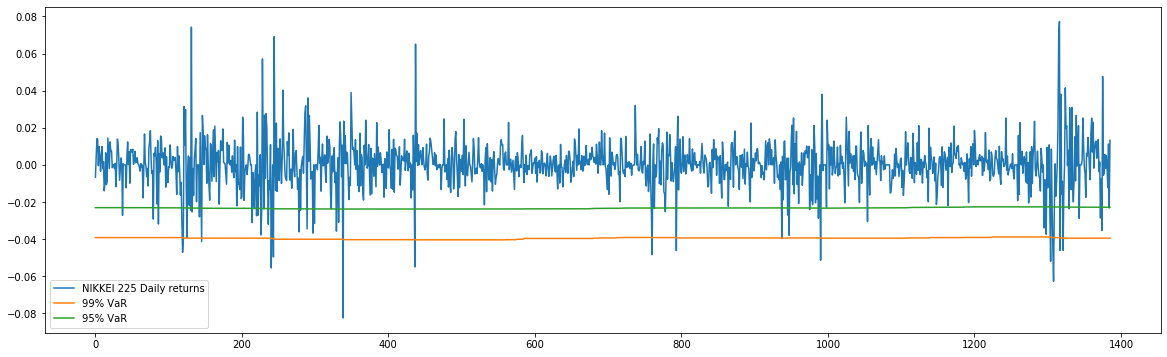
\includegraphics[width=0.8\textwidth]{figures/HISTN}
	\caption{Daily log-returns and daily VaR estimation of NIKKEI 225}
	\label{HistN}
\end{figure}


\begin{figure}[!h]
	\centering
	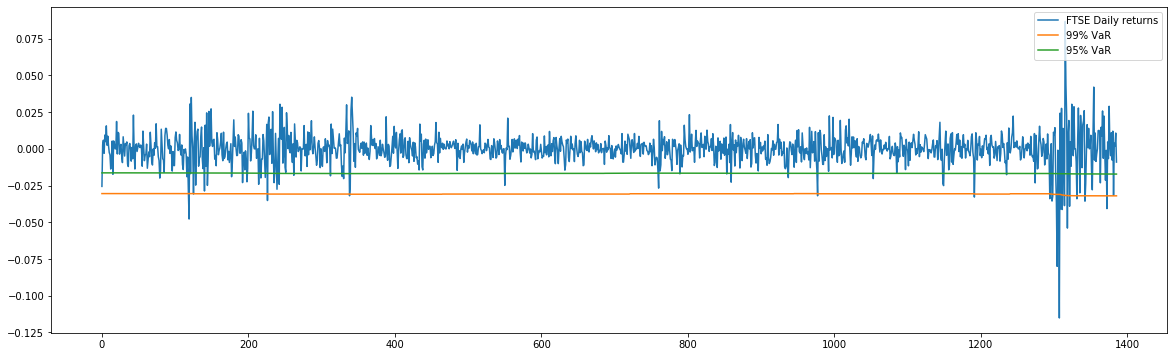
\includegraphics[width=0.8\textwidth]{figures/HISTF}
	\caption{Daily log-returns and daily VaR estimation of FTSE 100}
	\label{HistF}
\end{figure}

\begin{figure}[!h]
	\centering
	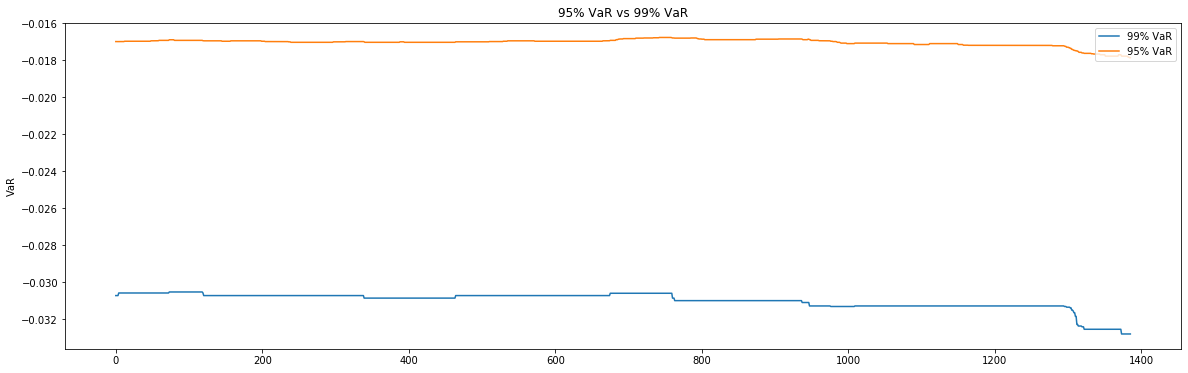
\includegraphics[width=0.8\textwidth]{figures/HISTS}
	\caption{Daily log-returns and daily VaR estimation of S\&P 500}
	\label{HistS}
\end{figure}
All the graphs (Fig 4.19 to Fig 4.21) clearly display presence of VaR violations. It can be observed that the Historical simulation reacts poorly to market changes as the movement of the plot seems to be constant.
\newpage
	\textbf{Garch(1,1)}
\begin{figure}[!h]
	\centering
	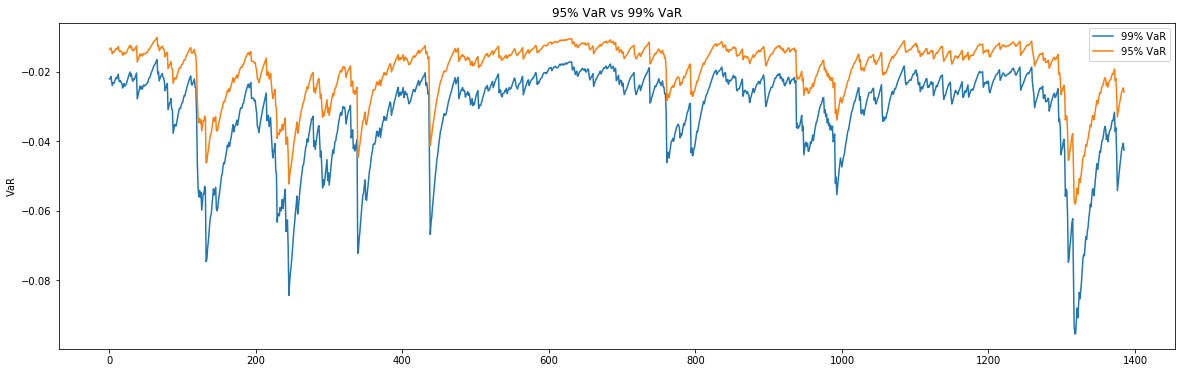
\includegraphics[width=0.8\textwidth]{figures/GARCHN}
	\caption{Daily log-returns and daily VaR estimation of NIKKEI 225}
	\label{garchN}
\end{figure}

\begin{figure}[!h]
	\centering
	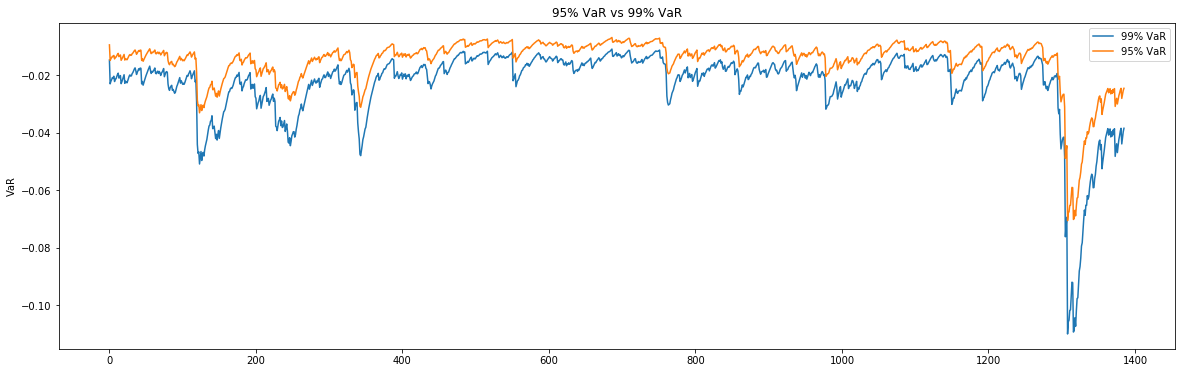
\includegraphics[width=0.8\textwidth]{figures/GARCHF}
	\caption{Daily log-returns and daily VaR estimation of FTSE 100}
	\label{garchF}
\end{figure}

\begin{figure}[!h]
	\centering
	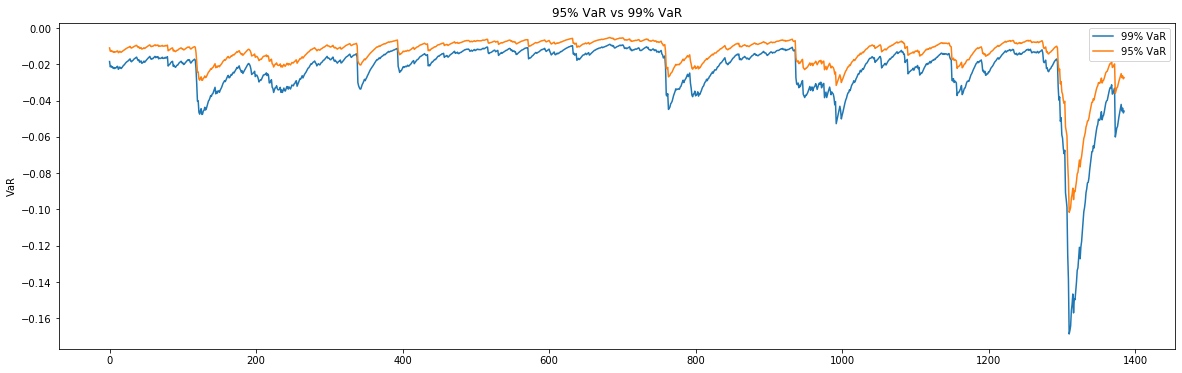
\includegraphics[width=0.8\textwidth]{figures/GARCHS}
	\caption{Daily log-returns and daily VaR estimation of S\&P 500}
	\label{garchS}
\end{figure}
All the graphs (Fig 4.22 to Fig 4.24) clearly display presence of VaR violations. The Garch (1,1) model seems to overreact when at the very extreme. When there is a very large loss, then there is a downward movement by the Garch model and then recovers quickly. Hence, it is not as stable as the Historical simulation as it seems to forget what has happened in the past.\\\\
\textbf{LSTM}	
\begin{figure}[!h]
	\centering
	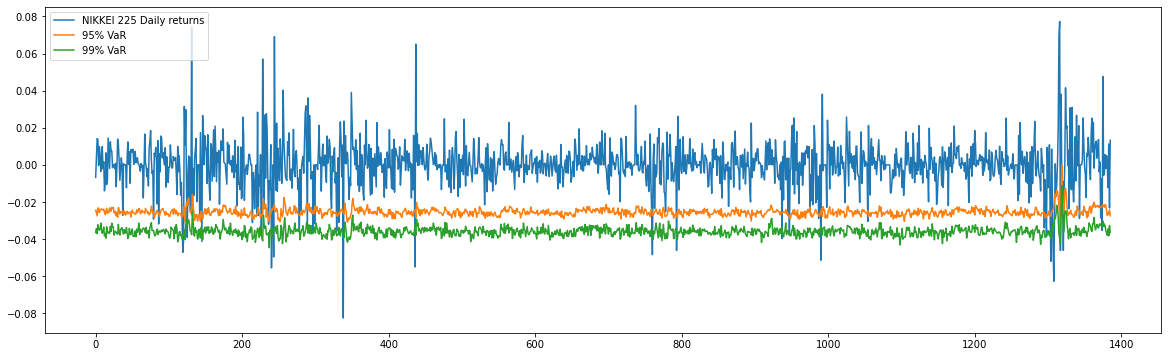
\includegraphics[width=0.8\textwidth]{figures/LSTMN}
	\caption{Daily log-returns and daily VaR estimation of NIKKEI 225}
	\label{LSTMN}
\end{figure}\\\\

\begin{figure}[!h]
	\centering
	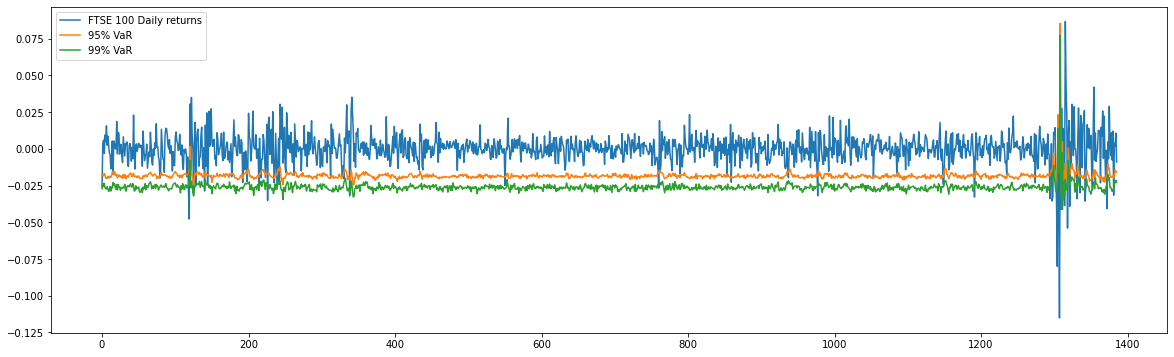
\includegraphics[width=0.8\textwidth]{figures/LSTMF}
	\caption{Daily log-returns and daily VaR estimation of FTSE 100}
	\label{LSTMF}
\end{figure}

\begin{figure}[!h]
	\centering
	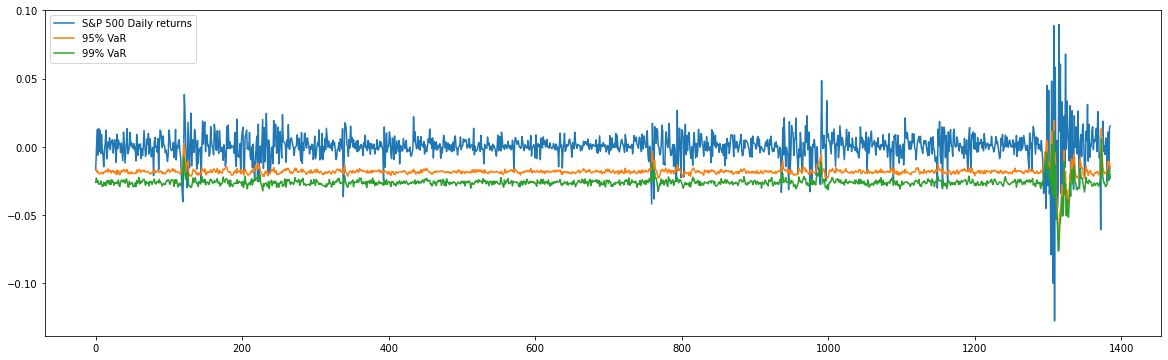
\includegraphics[width=0.8\textwidth]{figures/LSTMS}
	\caption{Daily VaR estimation of S\&P 500}
	\label{LSTMS}
\end{figure}	

All the graphs (Fig 4.25 to Fig 4.27) clearly display presence of VaR violations. The LSTM is more or less a mixture of Historical simulation and Garch (1,1) model. It is quite stable, but has some tiny movements which may be to the thousand simulation made for each individual day introduce some random errors, perhaps if we made a million simulation for each day the lstm model would be also be more flat or could maybe improve. Doing this requires huge computation time, which we are incapacitated to spend. The LSTM model is similar to Garch(1,1) as it reacts well to market movements.

	
\subsection{LSTM Volatility forecast}
Graphical representation of actual log-returns, LSTM predictions of the (mean) stock market log returns, and LSTM predictions of the (mean) stock market log returns with error term, are shown in this section. Observe that the three corresponding graphs for each stock market typically have a different scaling of the y-axis.\\\\
\textbf{NIKKEI 225}
\begin{figure}[!h]
	\centering
	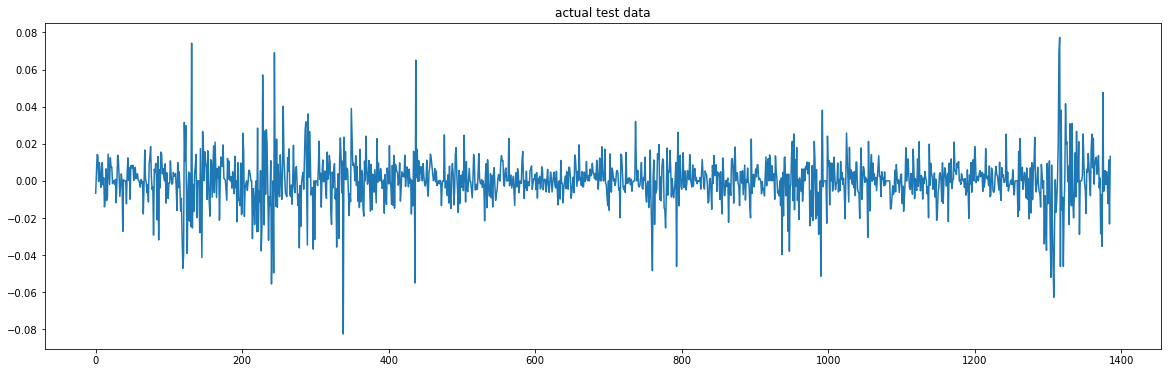
\includegraphics[width=0.8\textwidth]{figures/NIKKEITEST}
	\caption{Graphical display of NIKKEI 225 daily log-returns}
	\label{NIKKEITEST}
	

\end{figure}
\newpage
\begin{figure}[!h]
	\centering
	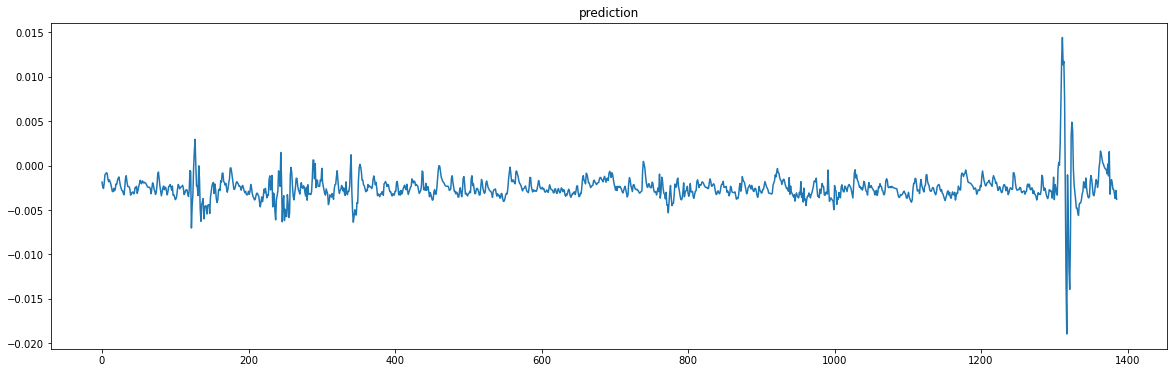
\includegraphics[width=0.8\textwidth]{figures/NIKKEIPRED}
	\caption{Graphical display of NIKKEI 225 predicted log-returns}
	\label{NIKKEIPRED}
\end{figure}


\begin{figure}[!h]
	\centering
	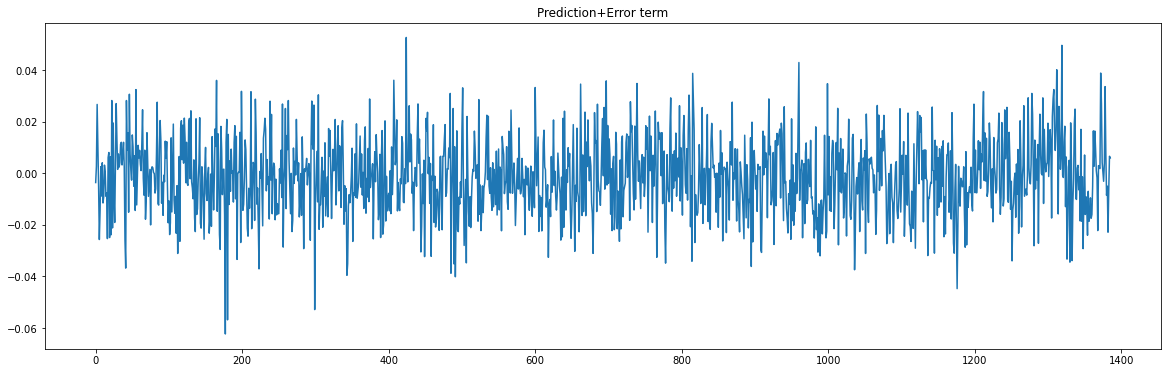
\includegraphics[width=0.8\textwidth]{figures/NIKKEIERROR}
	\caption{Graphical display of NIKKEI 225 predicted log-returns+Error term}
	\label{NIKKEIERROR}
\end{figure}
\autoref{NIKKEIERROR} do not show any market changes, probably due to random error.

\vfill


\textbf{FTSE 100}
\begin{figure}[!h]
	\centering
	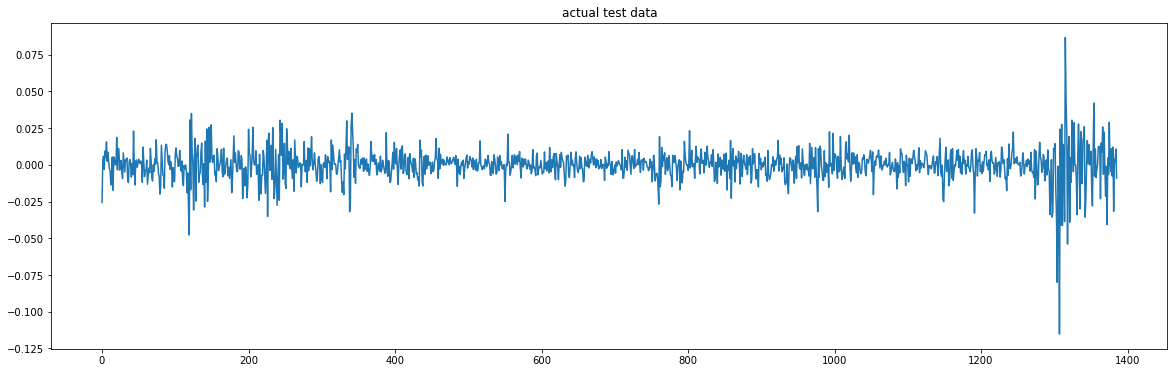
\includegraphics[width=0.8\textwidth]{figures/FTSETEST}
	\caption{Graphical display of FTSE 100 daily log-returns}
	\label{FTSETEST}
\end{figure}

\begin{figure}[!h]
	\centering
	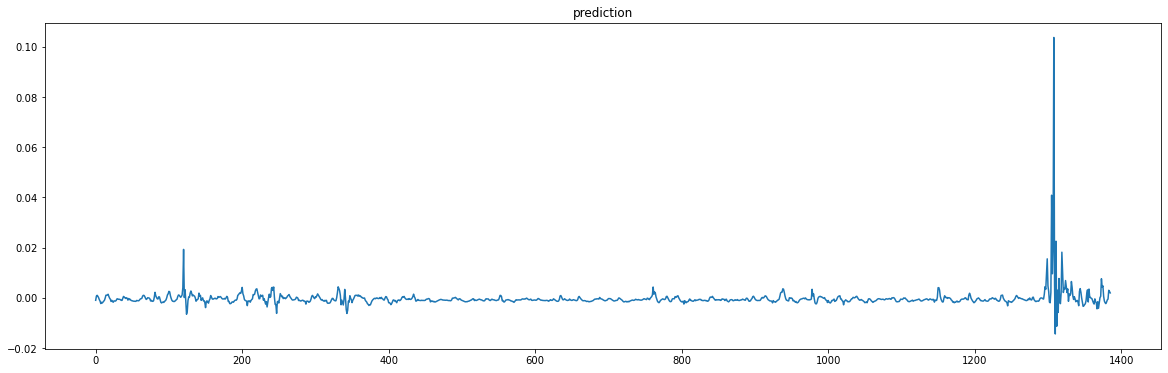
\includegraphics[width=0.8\textwidth]{figures/FTSEPRED}
	\caption{Graphical display of FTSE 100 predicted log-returns}
	\label{FTSEPRED}
\end{figure}


\begin{figure}[!h]
	\centering
	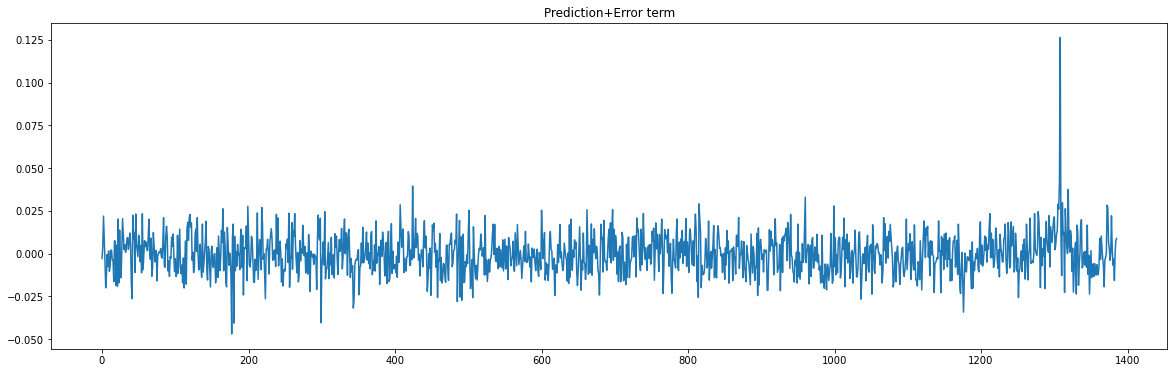
\includegraphics[width=0.8\textwidth]{figures/FTSEERROR}
	\caption{Graphical display of FTSE 100 predicted log-returns+Error term}
	\label{FTSEERROR}
\end{figure}
\newpage

\textbf{S\&P 500}

\begin{figure}[!h]
	\centering
	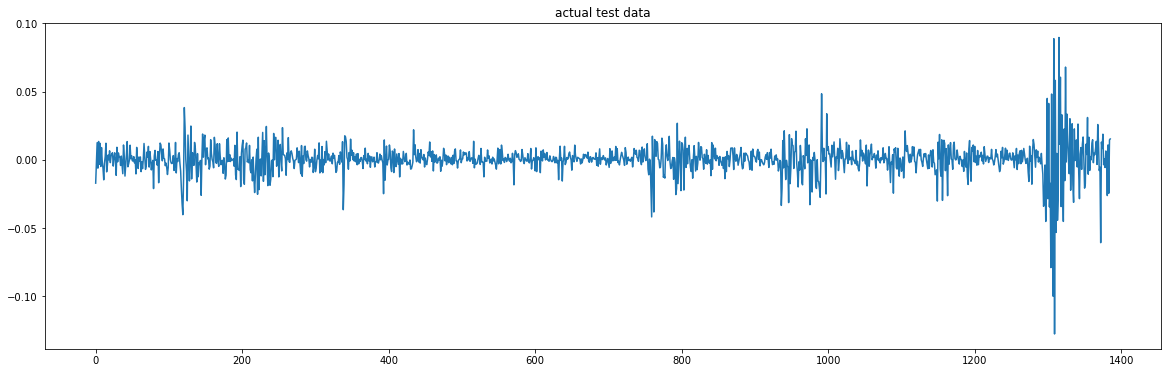
\includegraphics[width=0.8\textwidth]{figures/sanptest}
	\caption{Graphical display of S\&P 500 daily log-returns}
	\label{sanptest}
\end{figure}

\begin{figure}[!h]
	\centering
	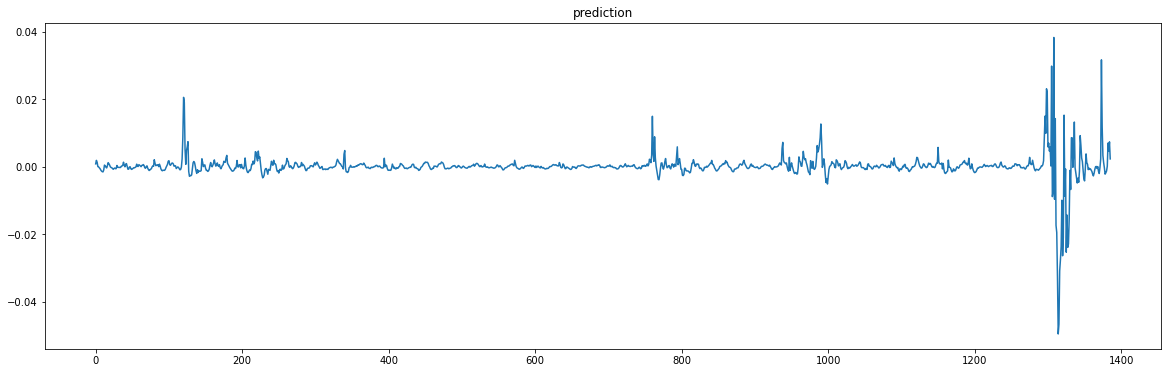
\includegraphics[width=0.8\textwidth]{figures/sanppred}
	\caption{Graphical display of S\&P 500 predicted log-returns}
	\label{sanpred}
\end{figure}


\begin{figure}[!h]
	\centering
	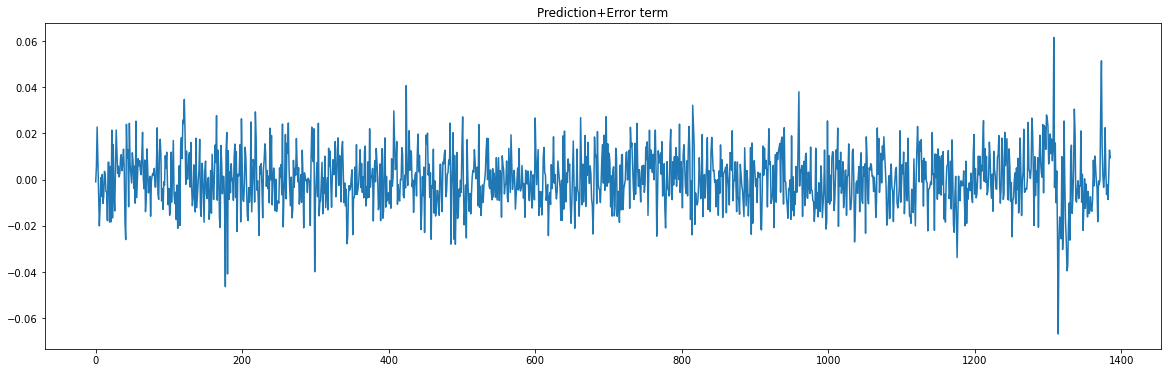
\includegraphics[width=0.8\textwidth]{figures/sanperror}
	\caption{Graphical display of S\&P 500 predicted log-returns+Error term}
	\label{sanpERROR}
\end{figure}
	From the graphs of the actual log-returns, it can be observed that the markets are quite stable with only small movements. The prediction graphs are more stable than that of the actual log-returns and shows quite great movements around the last few days.
	



\chapter{Conclusion}

From our Kupiec test, the Historical simulation performs best, followed by the Garch(1,1) and then, the LSTM model.\\\\  The historical simulation is stable, which is good in stable periods, but in periods when there is a lot of movements in the markets, its reaction is quite poor. It seems to have that as an advantage in this study, as our markets are quite stable over time, and they are quite traumatic at the final days, and in this period (final days) we have more VaR breaches.  Garch(1,1) and LSTM model react well to changes in market movement, particularly the Garch (1,1) model as it seems to be overoptimistic and overpessimistic sometimes. The LSTM model seems stable at stable periods and also react well to changes in market movement, so it may be seen as a more sensitive version of Historical simulation. All in all, we could say the performance of the models depend on the eventual movement of the markets.



%%%%%%%%%%%%%%%%%%%%%%%%%%%%%%%%%%%%%%%%%%%%%%%%%%%%%%%%%%%
%%%%%%%%%%%%%%%%%%%%%%%%%%%%%%%%%%%%%%%%%%%%%%%%%%%%%%%%%%%
%%%%%%%%%%%%%%%%%%%%%%%%%%%%%%%%%%%%%%%%%%%%%%%%%%%%%%%%%%%


%%%%%%%%%%%%%%%%%%%%%%%%%%%%%%%%%%%%%%%%%%%%%%%%%%%%%%%%%%%
%%%%%%%%%%%%%%%%%%%%%%%%%%%%%%%%%%%%%%%%%%%%%%%%%%%%%%%%%%%
%%%%%%%%%%%%%%%%%%%%%%%%%%%%%%%%%%%%%%%%%%%%%%%%%%%%%%%%%%%



	%%%%%%%%%%%%%%%%%%%%%%%%%%%%%%%%%%%%%%%%%%%%%%%%%%%%%%%%%%%
	%%%%%%%%%%%%%%%%%%%%%%%%%%%%%%%%%%%%%%%%%%%%%%%%%%%%%%%%%%%



	%%%%%%%%%%%%%%%%%%%%%%%%%%%%%%%%%%%%%%%%%%%%%%%%%%%%%%%%%%%
	



	
	
	






	%%%%%%%%%%%%%%%%%%%%%%%%%%%%%%%%%%%%%%%%%%%%%%%%%%%%%%%%%%%\\
	%%%%%%%%%%%%%%%%%%%%%%%%%%%%%%%%%%%%%%%%%%%%%%%%%%%%%%%%%%%
	

	
	%%%%%%%%%%%%%%%%%%%%%%%%%%%%%%%%%%%%%%%%%%%%%%%%%%%%%%%%%%%


%%%%%%%%%%%%%%%%%%%%%%%%%%%%%%%%%%%%%%%%%%%%%%%%%%%%%%%%%%%
%%%%%%%%%%%%%%%%%%%%%%%%%%%%%%%%%%%%%%%%%%%%%%%%%%%%%%%%%%%
%%%%%%%%%%%%%%%%%%%%%%%%%%%%%%%%%%%%%%%%%%%%%%%%%%%%%%%%%%%

\bibliographystyle{plain}
\bibliographystyle{abbrvnat}
\bibliography{literature/library}
Acerbi, C. and Tasche, D. On the coherence of expected shortfall, \textit{Journal of Banking and Finance}, Vol. 26, 2002,
pp. 1496-1500.\newline\newline
Corsi, F. (2009). A simple approximate long-memory model of realized volatility, \textit{Journal of
Financial Economic}, 7(2), 174-196.\newline\newline 
Jorion, P. Value at Risk: The New Benchmark for Managing Financial Risk, McGraw-Hill, 2007.\newline\newline
Sun, W., Rachev, S., Chen, Y and Fabozzi, F., (2008). Measuring Intra-Day Market
Risk: A Neural Network Approach.\newline\newline
James W. Taylor (2019). Forecasting Value at Risk and Expected Shortfall
Using a Semiparametric Approach Based on the Asymmetric Laplace Distribution, \textit{Journal of
Business \& Economic Statistics}, 37:1, 121-133.\newline\newline
Patton, A.J., Ziegel, J.F., Chen, R. (2019). Dynamic semiparametric models for expected shortfall
(and Value-at-Risk), \textit{Journal of Econometrics}, 211, 388-413.\newline\newline
Arimond A., et al (2020). Neural Networks and Value at Risk. 	arXiv:2005.01686\newline\newline
Nagai M. (2016) Estimation of Extreme Value at Risks Using CAViaR Models, \textit{Graduate School of Economics, Hitotsubashi University}.\newline\newline
Abed, P., Benito, S., (2013). A detailed comparison of value at risk estimates, \textit{Mathematics and Computers in Simulation}, 94, 258–276.\newline\newline
Abed, P., Benito, S., (2009). A Detailed Comparison of Value at Risk in International Stock Exchanges\newline\newline
Graves, A. (2013). Generating sequences with recurrent neural networks. arXiv preprint arXiv:1308.0850.\newline\newline
Abed, P., Benito, S., Lopez, C. A comprehensive review of Value at Risk methodologies, \textit{Spanish Review of Financial Economics} 12(1), 2013. \\\\
Ruilova, J.C., Morettin P. A., (2020). Parsimonious Heterogeneous ARCH Models for High
Frequency Modeling, \textit{Journal of Risk and Financial Management}.\\\\
Yu, P., Yan, X. Stock price prediction based on deep neural networks, \textit{Journal of Neural Computing and Applications} 32(5), 2020.\\\\
Buczyński, Mateusz; Chlebus, Marcin (2018) : Comparison of semiparametric
and benchmark value-at-risk models in several time periods with different volatility
levels, \textit{e-Finanse: Financial Internet Quarterly, ISSN 1734-039X, University of Information
Technology and Management, Rzeszów, Vol. 14, Iss. 2, pp. 67-82,
http://dx.doi.org/10.2478/fiqf-2018-0013}\\\\
Bijelic \& Ouijjane (2019) : Predicting Exchange Rate
Value-at-Risk and Expected Shortfall:
A Neural Network Approach. \textit{Master thesis, School of Economics and Management, Lund University}.\\\\
Kingma, D. and Ba, J. (2015) Adam: A Method for Stochastic Optimization. \textit{Proceedings of the 3rd International Conference on Learning Representations (ICLR 2015)}.\\\\
Teo Li Hui (2006) : Comparison of Value-At-Risk (VAR) Using Delta-Gamma
Approximation with Higher Order Approach. \textit{Master thesis, Department of Mathematics, National University of Singapore}.\\\\
James W. Taylor (2020). Forecast combinations for value at risk and expected shortfall, \textit{International Journal of Forecasting}, 36, 428-441.\\\\
Chaoyi Lou (2019). Artificial Neural Networks:
their Training Process and Applications \textit{Department of Mathematics, Whitman College}.\\\\
IBM (2020). Neural Networks, https://www.ibm.com/cloud/learn/neural-networks\\\\
IBM (2020). Recurrent Neural Networks, https://www.ibm.com/cloud/learn/recurrent-neural-networks\\\\
Brownlee, J., (2016). Time Series Prediction with LSTM Recurrent Neural Networks
in Python with Keras, Deep Learning for time series.\\\\
Locarek-Junge, H. and Prinzler, R. (1999). Using ANN to Estimate VaR, working
paper.\\\\
S. A. Hamid and Z. Iqbal. Using neural networks for forecasting volatility of S\&P 500 Index futures prices \textit{Journal of Business Research 57 (2004) 1116–1125}.\\\\
He, K., Ji, L., Tso, G. K. F., Zhu, B., \& Zou, Y. (2018). Forecasting Exchange Rate Value at Risk using Deep Belief Network Ensemble based Approach. \textit{Procedia Computer Science}, 139, 25-32.
https://doi.org/10.1016/j.procs.2018.10.213.\\\\
K. Hornik, M. Stinchcombe, H. White. Multilayer Feedforward Networks are Universal Approximators , Vol. 2, pp. 35Y-366, 1989
Peter Kretschmer (2019): Neural Hawkes Processes with Applications
in Finance. \textit{Master thesis, Department of Mathematics, Technische Universität Kaiserslautern}.\\\\
Tenti, P. (1996). Forecasting foreign exchange rates using recurrent neural networks. Taylor \& Francis.\\\\
Fabian Kremer, 2013, Concept of Value at Risk (VaR), Munich, GRIN Verlag.



\listoffigures
\listoftables

%\printindex
\begin{appendix}
	\chapter{}
	
	Here you find the pictorial view of the main python programming codes used for our computations. Codes are run in Jupyter notebook environment.
	\begin{figure}[!h]
		\centering
		\includegraphics[width=0.8\textwidth]{figures/code1}
		\caption{Python codes for Historical simulation}
	
	\end{figure}
	
	\begin{figure}[!h]
		\centering
		\includegraphics[width=0.8\textwidth]{figures/code2}
		\caption{Python codes for Garch (1,1)}
	\end{figure}
	
	\begin{figure}[!h]
		\centering
		\includegraphics[width=0.8\textwidth]{figures/code3}
		\caption{Python codes for LSTM architecture}
	\end{figure}
	 \vspace{50mm}
	\begin{figure}[!h]
		\centering
		\includegraphics[width=0.8\textwidth]{figures/code4}
		\caption{Python codes for LSTM VaR model}
	\end{figure}

	
	
\end{appendix}

%%%%%%%%%%%%%%%%%%%%%%%%%%%%%%%%%%%%%%%%%%%%%%%%%%%%%%%%%%%
%%%%%%%%%%%%%%%%%%%%%%%%%%%%%%%%%%%%%%%%%%%%%%%%%%%%%%%%%%%
%%%%%%%%%%%%%%%%%%%%%%%%%%%%%%%%%%%%%%%%%%%%%%%%%%%%%%%%%%%


%%%%%%%%%%%%%%%%%%%%%%%%%%%%%%%%%%%%%%%%%%%%%%%%%%%%%%%%%%%
%%%%%%%%%%%%%%%%%%%%%%%%%%%%%%%%%%%%%%%%%%%%%%%%%%%%%%%%%%%
%%%%%%%%%%%%%%%%%%%%%%%%%%%%%%%%%%%%%%%%%%%%%%%%%%%%%%%%%%%



%%%%%%%%%%%%%%%%%%%%%%%%%%%%%%%%%%%%%%%%%%%%%%%%%%%%%%%%%%%
%%%%%%%%%%%%%%%%%%%%%%%%%%%%%%%%%%%%%%%%%%%%%%%%%%%%%%%%%%%








%%%%%%%%%%%%%%%%%%%%%%%%%%%%%%%%%%%%%%%%%%%%%%%%%%%%%%%%%%%
%%%%%%%%%%%%%%%%%%%%%%%%%%%%%%%%%%%%%%%%%%%%%%%%%%%%%%%%%%%
%%%%%%%%%%%%%%%%%%%%%%%%%%%%%%%%%%%%%%%%%%%%%%%%%%%%%%%%%%%
\end{document}

%%%%%%%%%%%%%%%%%%%%%%%%%%%%%%%%%%%%%%%%%%%%%%%%%%%%%%%%%%%
